%%%%%
%%%%%  Use LUALATEX, not LATEX.
%%%%%
%%%%
\documentclass[]{VUMIFTemplateClass}

\usepackage{indentfirst}
\usepackage{amsmath, amsthm, amssymb, amsfonts}
\usepackage{mathtools}
\usepackage{bm}
\usepackage{physics}
\usepackage{graphicx}
\usepackage{verbatim}
\usepackage[hidelinks]{hyperref}
\usepackage{color,algorithm,algorithmic}
\usepackage[nottoc]{tocbibind}
\usepackage{tocloft}
\usepackage{booktabs}
\usepackage{multirow}
\usepackage{caption}
\usepackage{subcaption}
\usepackage{tikz}
\usetikzlibrary{shapes,arrows,positioning}

\usepackage{titlesec}
\newcommand{\sectionbreak}{\clearpage}

\makeatletter
\renewcommand{\fnum@algorithm}{\thealgorithm}
\makeatother
\renewcommand\thealgorithm{\arabic{algorithm} algorithm}

\usepackage{biblatex}
\bibliography{bibliografija}
%% to change the numbering (numeric or alphabetic) of bibliographic sources, make the change in VUMIFTemplateClass.cls, line 139

% Author's MACROS
\newcommand{\EE}{\mathbb{E}\,} % Mean
\newcommand{\ee}{{\mathrm e}}  % nice exponent
\newcommand{\RR}{\mathbb{R}}

\studyprogramme{Data Science}
\worktype{Master's thesis}
\worktitle{Training Data Selection Strategies for Multi-Speaker Text-to-Speech Synthesis in Lithuanian}
\secondworktitle{Mokymo duomenų parinkimo strategijos šnekos sintezės modelio apmokymui lietuvių kalba, naudojant kelių kalbėtojų balsus}
\workauthor{Aleksandr Jan Smoliakov}

\supervisor{Dr.~Gerda Ana Melnik-Leroy}
\reviewer{pedagogical/scientific title Name Surname}
\scientificadvisor{Prof.~Dr.~Gražina Korvel}

\begin{document}
\selectlanguage{english}

\onehalfspacing
\input{TitlePage}

\sectionnonum{Summary}

Developing high-quality Text-to-Speech (TTS) systems for low-resource languages
is often hindered by a lack of large, single-speaker datasets. This thesis
investigates training data composition strategies for Lithuanian multi-speaker
TTS models, specifically testing the hypothesis that data depth is critical for
synthesis quality. Using the Liepa-2 corpus, three datasets were constructed
with a constant total duration of 22.5 hours, varying the trade-off between
breadth (30 to 180 speakers) and depth (45 to 7.5 minutes per speaker).
Tacotron 2 and Glow-TTS architectures were trained and evaluated via objective
metrics (MCD, F0 RMSE) and subjective listening tests (MOS). Results
demonstrate that Tacotron 2 consistently outperforms Glow-TTS in naturalness.
Contrary to the hypothesis, statistical analysis reveals no significant
difference in synthesis quality across the varying data strategies. This
suggests that modern multi-speaker models are insensitive to the breadth-depth
trade-off within this range, achieving convergence with as little as 7.5
minutes of data per speaker.

\textbf{Keywords:} text-to-speech, multi-speaker
voice synthesis, low-resource language, Tacotron 2, Glow-TTS

\sectionnonum{Santrauka}

Aukštos kokybės šnekos sintezės (TTS) sistemų kūrimą mažai išteklių turinčioms
kalboms dažnai sunkina didelių vieno kalbėtojo duomenų rinkinių trūkumas. Šiame
darbe tiriamos mokymo duomenų parinkimo strategijos šnekos sintezės modelio
apmokymui lietuvių kalba, naudojant kelių kalbėtojų balsus. Tikrinama iškelta
hipotezė, kad duomenų gylis yra kritiškai svarbus sintezės kokybei. Naudojant
Liepa-2 garsyną, sudaryti trys duomenų rinkiniai, kurių bendra trukmė yra
pastovi (22,5 val.), tačiau kinta santykis tarp duomenų pločio (nuo 30 iki 180
kalbėtojų) ir gylio (nuo 45 iki 7,5 min.\ vienam kalbėtojui). Apmokytos
Tacotron 2 ir Glow-TTS architektūros bei atliktas jų vertinimas, panaudojant
objektyvius rodiklius (MCD, F0 RMSE) ir subjektyvius klausymo testus (MOS).
Rezultatai rodo, kad Tacotron 2 pagal natūralumą nuosekliai lenkia Glow-TTS\@.
Statistinė analizė paneigė iškeltą hipotezę ir neatskleidė reikšmingo sintezės
kokybės skirtumo taikant skirtingas duomenų strategijas. Tai leidžia teigti,
kad šiuolaikiniai kelių kalbėtojų modeliai šiame intervale nėra jautrūs pločio
ir gylio santykiui ir geba konverguoti turint vos 7,5 minutės duomenų vienam
kalbėtojui.

\textbf{Raktiniai žodžiai:} šnekos sintezė, kelių kalbėtojų balsų sintezė, mažai išteklių turinti kalba, Tacotron 2, Glow-TTS

\singlespacing
\selectlanguage{english}

% list of figures, delete if not needed
\listoffigures

% list of tables, delete if not needed
\listoftables

% Table of contents
\tableofcontents
\onehalfspacing

%%%%%%%%%%%%%%%%%%%%%%%%%%%%%%%%%%%%%%%%%%%%%%%%%%%%%%%%%%%%%%%%%%%%%%%%%%%%%%%%
%% Introduction
%%%%%%%%%%%%%%%%%%%%%%%%%%%%%%%%%%%%%%%%%%%%%%%%%%%%%%%%%%%%%%%%%%%%%%%%%%%%%%%%
\sectionnonum{Introduction}

The goal of creating machines that can speak like humans has captivated
researchers for centuries. One of the earliest known attempts dates back to the
18th century, with Wolfgang von Kempelen's mechanical ``speaking
machine''~\cite{dudley1950speaking} that utilized a bellows-driven lung and
physical models of the tongue and lips to produce rudimentary speech sounds.

Over the centuries, our understanding of human speech and advancements in
technology have driven significant progress in this field. Today's
state-of-the-art Text-to-Speech (TTS) systems, dominated by end-to-end (E2E)
neural models such as Tacotron~2~\cite{shen2018natural} and
Glow-TTS~\cite{kim2020glowtts}, have achieved highly natural speech with
unprecedented acoustic quality. Notably, these E2E systems have unified the
entire synthesis process into one or two neural networks, learning to map text
inputs (graphemes or phonemes) directly to audio outputs, eliminating the need
for complex, brittle multi-stage pipelines.

These advancements have transformed TTS from a niche area of academic curiosity
into essential tools for daily life. High-quality speech synthesis now powers
popular virtual assistants~\cite{hoy2018alexa} and navigation systems, serving
as a primary interface for human-computer interaction. More importantly, it
plays a critical role in accessibility, enabling screen readers for the
visually impaired~\cite{isewon2014design, taylor2009text}, providing a voice
for the non-verbal, and facilitating access to
information~\cite{taylor2009text}.

However, the transition to deep learning techniques has introduced a new
dependency: data. While modern neural TTS models are capable of producing
remarkably natural speech, they lack explicit linguistic prior knowledge,
making them heavily reliant on large amounts of high-quality training data to
learn implicit mappings from text to speech. The common recommendation is to
use at least 10 to 20~hours of high-quality recorded speech from a single
speaker to achieve good synthesis quality. The majority of existing research
and commercial TTS systems focus on high-resource languages like English, where
professionally recorded single-speaker datasets (e.g.,
LJSpeech~\cite{ljspeech17} with 24 hours of speech) are readily available.

However, low-resource languages, such as Lithuanian, often lack such extensive
datasets, and available corpora tend to be crowd-sourced with multiple speakers
contributing small amounts of data each. In contrast, multi-speaker TTS models
can achieve convergence and reasonable intelligibility with significantly less
data per speaker --- as little as 15 to 30 minutes --- provided the total
pooled dataset is sufficiently large to learn the language's phonetics and
prosody.

Liepa-2~\cite{liepa2project} is a Lithuanian speech corpus, released in 2020,
that contains 1000~hours of annotated speech; this data is distributed across
2621~speakers, with most speakers contributing under 30~minutes each. The top
speaker has under 2.5~hours of recorded speech, well below the standard
recommendation for training a high-fidelity single-speaker TTS model.

Having such a fragmented dataset, or crowd-sourced data, presents an
engineering challenge. Using a single speaker's data from such a corpus yields
insufficient data for high-quality synthesis. On the other hand, training on
the entire 1000-hour corpus is a computationally prohibitive process for the
scope of this work. Therefore, a multi-speaker TTS architecture is the
necessary solution. It allows for the aggregation of data from a selected
subset of speakers, provided the model can learn to disentangle speaker
identity from shared linguistic features.

This necessitates a choice between two competing strategies under a fixed
computational budget: prioritizing \textbf{breadth} (many speakers with little
data each) or \textbf{depth} (fewer speakers with more data each).
Consequently, the question that arises is: \textit{what is the optimal strategy
      for sampling multi-speaker data to maximize synthesis quality?}

Current literature generally advocates for transfer learning from large
pre-trained models to improve low-resource TTS performance. However, there is a
lack of research specifically addressing the internal composition of the
training set for morphologically complex languages like Lithuanian. To address
this gap and isolate the effects of data distribution without the bias of
pre-training, this thesis investigates the optimal data selection strategy for
training Lithuanian multi-speaker TTS models from scratch.

The primary \textbf{research aim} of this thesis is to: measure how varying the
balance between training dataset \textit{breadth} (number of speakers) and
\textit{depth} (duration per speaker) affects the synthesis quality of
multi-speaker TTS models. The \textbf{hypothesis} is that depth is a more
critical factor --- more specifically, that synthesis quality will degrade as
the number of speakers increases, given a constant total training duration.

To achieve this aim, the following \textbf{research objectives} are defined:

\begin{itemize}
      \item Process the Liepa-2 dataset to prepare three TTS training datasets that
            maintain a constant total duration but vary in speaker distribution.
      \item Configure and train two distinct acoustic model architectures (one
            autoregressive, one non-autoregressive) on each of the created datasets.
      \item Evaluate the synthesis quality of the trained models using objective metrics.
      \item Develop a subjective evaluation application and conduct a Mean Opinion Score
            listening test with native Lithuanian speakers to assess naturalness.
\end{itemize}

The remainder of this thesis is organized as follows: The \textbf{Literature
      Review} presents an overview of relevant concepts in digital signal processing,
neural TTS architectures, and the specific challenges of Lithuanian TTS\@.
\textbf{Methodology} describes the data selection, model configurations, and
experimental design. \textbf{Results} presents the findings of the objective
and subjective synthesis quality evaluations, analyzing the failure modes of
the models. Finally, the \textbf{Conclusion} summarizes the key findings and
offers potential recommendations for future research in low-resource TTS
synthesis.

%%%%%%%%%%%%%%%%%%%%%%%%%%%%%%%%%%%%%%%%%%%%%%%%%%%%%%%%%%%%%%%%%%%%%%%%%%%%%%%%
%% Literature review
%%%%%%%%%%%%%%%%%%%%%%%%%%%%%%%%%%%%%%%%%%%%%%%%%%%%%%%%%%%%%%%%%%%%%%%%%%%%%%%%
\section{Literature Review}

This section reviews the key concepts related to text-to-speech synthesis and
traces the evolution from traditional methods to modern neural architectures.
The topics are presented in a bottom-up manner, building up from fundamental
signal processing concepts to high-level TTS architectures.

\subsection{Digital Representation of Audio}

At its core, the objective of a TTS system is to generate an audio signal --- a
continuous pressure wave --- that the human ear perceives as speech. The key
properties of sound waves include frequency (pitch), amplitude (loudness), and
phase. However, digital audio processing, as used in TTS systems, requires
converting sound waves into a discrete digital format. This conversion involves
two main steps: sampling and quantization.

Sampling is the process of measuring the amplitude of the sound wave at regular
time intervals. The rate at which these samples are taken is called the
sampling rate. Increasing the sampling rate allows for capturing higher
frequency components of the audio signal; however, it also increases the amount
of data that needs to be processed and stored. Thus, there is a trade-off
between audio quality and data efficiency. According to the
Nyquist-Shannon~\cite{shannon1949communication} sampling theorem, accurate
reconstruction of a continuous signal requires a sampling rate that is strictly
greater than twice the highest frequency present in the signal. While
frequencies in the range of 300~Hz to 3400~Hz contribute most to human speech
intelligibility and recognition~\cite{jothilakshmi2016large}, high-fidelity
synthesis typically uses sampling rates of 22.05~kHz and 24~kHz, which can
capture frequencies up to approximately 11~kHz and 12~kHz, respectively.

Quantization (or bit depth) is the mapping of continuous amplitude values to
discrete levels for digital representation, which determines the precision of
the representation. Similar to sampling rate, there is a trade-off between
audio quality and data size. Common bit depths for audio are 16-bit and 24-bit
formats. A visual representation of both sampling and quantization is provided
in Figure~\ref{fig:sampling}.

\begin{figure}[ht]
      \centering
      \includegraphics[width=\textwidth]{figures/sampling_quantization.pdf}
      \caption[Visual representation of Analog-to-Digital conversion]{Visual representation of Analog-to-Digital conversion. The continuous grey line represents the analog signal. The vertical lines represent the \textbf{sampling rate} (time intervals), and the horizontal grid lines represent \textbf{quantization levels} (bit depth).}\label{fig:sampling}
\end{figure}

In neural TTS systems, which typically operate on frequency-domain
representations like Mel-spectrograms (discussed below), \textbf{Pre-Emphasis}
is a common audio pre-processing step applied to the raw waveform. Natural
speech signals tend to have more energy in the lower frequencies, with a
gradual drop-off towards higher frequencies (approximately -6~dB per octave).
This spectral tilt can lead to models focusing disproportionately on
low-frequency components, potentially neglecting important high-frequency
details. Pre-emphasis compensates for this spectral tilt by boosting high
frequencies using a first-order high-pass filter, which is defined as:

\begin{equation}
      y[n] = x[n] - \alpha x[n-1]
\end{equation}

where \( y[n] \) is the pre-emphasized signal, \( x[n] \) is the original
signal, \( \alpha \) is the pre-emphasis coefficient (typically between 0.9 and
1.0, and often set to 0.97), and \( n \) is the sample index.

This improves the signal-to-noise ratio for high frequencies and prevents the
model from neglecting higher-frequency components.

\subsection{Time-Frequency Analysis}

\subsubsection*{Fourier Transform}

TTS systems typically do not operate directly on the raw waveform. Instead,
they rely on time-frequency representations that capture the spectral content
of the signal over time.

The \textbf{Fourier Transform} (FT) is a mathematical technique that transforms
a time-domain signal (such as an audio waveform) into its frequency-domain
representation. The signal is decomposed into a sum of sine and cosine waves at
various frequencies, each with a specific amplitude and phase. This allows us
to analyze the frequency content of the signal.

The \textbf{Short-Time Fourier Transform} (STFT)~\cite{gabor1946theory} extends
the FT by applying it to short, overlapping segments (frames) of the signal.
This transformation provides a time-frequency representation, showing how the
frequency content of the signal changes over time --- precisely the features
needed for modeling speech.

In TTS applications, the STFT is computed by dividing the audio signal into
short frames (usually 20--50~ms) with a certain overlap (usually 50--75\%)
between frames, windowed by a Hamming or Hann function to reduce spectral
leakage.

\subsubsection*{Spectrogram and Mel-Spectrogram}

The \textbf{spectrogram} is a visual representation of the STFT, displaying
frequency on the vertical axis, time on the horizontal axis, with amplitude
represented by color intensity. In TTS systems, spectrogram values are the
typical intermediate representation between an acoustic model and a vocoder
(discussed later) --- the spectrogram being the target output of the acoustic
model.

The regular spectrogram uses a linear frequency scale. While it allows a
detailed frequency analysis, this has limitations when modeling human speech.
The human ear does not perceive frequencies linearly --- it is more sensitive
to pitch differences at lower frequencies than higher ones. To mimic this
perceptual characteristic, the Mel scale~\cite{stevens1937scale} maps linear
frequency \( f \) (in Hz) to a perceptual scale \( m \) (in Mels) using the
following formula:

\begin{equation}
      m = 2595 \cdot \log_{10}\left(1 + \frac{f}{700}\right)
\end{equation}

\textbf{Mel-spectrograms} are computed by applying a Mel filterbank of overlapping
triangular filters (spaced uniformly on the Mel scale) to the magnitude spectrogram obtained from the STFT\@.
Finally, the dynamic range of the amplitudes is compressed by taking the
logarithm (usually resulting in decibels), as human loudness perception is
logarithmic. This results in a compressed representation of the audio signal
that aligns more closely with human auditory perception. Such Mel-spectrograms
are commonly used as input features for modern TTS systems. The differences
between the raw waveform, the standard spectrogram, and the Mel-spectrogram are
illustrated in Figure~\ref{fig:waveform_spectrograms}. Note how the
Mel-spectrogram has a higher resolution in the lower frequencies, where the
majority of speech energy is concentrated.

\begin{figure}[ht]
      \centering
      \includegraphics[width=\textwidth]{figures/waveform_spectrograms.pdf}
      \caption[Raw waveform, Spectrogram, and Mel-spectrogram]{Raw audio waveform (top), its linear frequency spectrogram (middle), and Mel-spectrogram (bottom) representations for the utterance ``Štai ir visas mano bendravimas su vaiku''.}\label{fig:waveform_spectrograms}
\end{figure}

It is important to note that converting a waveform to a Mel-spectrogram is
lossy: phase information is discarded during the magnitude operation, and
frequency resolution is reduced by the Mel filterbank. As a result,
reconstructing a high-fidelity audio waveform from a generated Mel-spectrogram
requires a specialized model component, typically referred to as a vocoder
(discussed in Section~\ref{sec:vocoder}).

\subsection{Linguistic Representation}

In TTS systems, the input text must be pre-processed and converted into a
suitable linguistic representation that the synthesis model can use. Although
theoretically an end-to-end TTS model could learn to map raw text directly to
audio, in practice, pre-processing the text facilitates model convergence and
improves the quality of the synthesized speech.

The main goal of this stage is to map the raw sentences into a sequence of
symbols that can be more closely mapped to the acoustic features of speech.
This process typically involves several steps, such as text normalization,
grapheme-to-phoneme conversion, and possibly prosody prediction.

\subsubsection{Text Normalization}

Text normalization~\cite{sproat2001normalization} is the process of converting
raw written text with non-standard words into a more standardized ``spoken''
form. Typical steps include expanding abbreviations (e.g., expanding ``Dr.'' to
``Doctor''), punctuation standardization, number normalization (e.g.,
converting ``123'' to ``one hundred twenty-three''), and lowercasing. While
some non-standard punctuation is removed, structural punctuation (commas,
periods) is often retained or mapped to special pause tokens to guide prosody.
As an example, the input text ``Dr.\ Smith has 2 cats.'' could be normalized to
``doctor smith has two cats'', which bears closer resemblance to the spoken
form.

Text normalization helps reduce the variability and complexity in the input
text, decreases the number of unique symbols, and removes the ambiguities that
could confuse the TTS model. The resulting normalized text is not only easier
for the model to process, but can also be further converted into phonemes,
which provide an even closer representation of spoken language.

\subsubsection{Graphemes versus Phonemes}

Text-to-speech systems use a discrete input representation derived from text,
generally divided into grapheme-based or phoneme-based sequences.

Grapheme-based models ingest raw character sequences (orthography). This
approach simplifies the inference pipeline by eliminating the dependency on
external grapheme-to-phoneme (G2P) converters. However, it forces the model to
implicitly learn pronunciation rules from data, which can be a significant
challenge for languages with complex orthographies or heteronyms (e.g., English
``read'' /riːd/ and ``read'' /rɛd/, depending on the tense).

In contrast, the phoneme-based approach uses a phonetic transcription of the
text, typically in the International Phonetic Alphabet or ARPABET form. By
resolving pronunciation ambiguities prior to training, phonemes provide a more
direct mapping to acoustic features, simplifying the model's task of learning
alignment. The downside is that this approach requires an external G2P
conversion step~\cite{bisani2008joint}. Additionally, errors in the G2P
conversion can propagate to the TTS model, affecting the quality of the
synthesized speech.

For languages with highly regular orthographies (e.g., Spanish, Lithuanian),
there is another approach that augments the grapheme-based representation with
explicit lexical stress markers (e.g., tilde, acute, grave accents). This
intermediate method helps the model disambiguate pronunciation of homographs
and learn prosodic patterns more easily without requiring a full phonetic
transcription, particularly in languages where stress placement alters meaning.

\subsubsection{Challenges in Lithuanian TTS}

Lithuanian is a Baltic language with rich inflectional morphology and a complex
prosodic structure. It is a pitch-accent language with free stress, meaning the
stress can fall on any syllable in a word, and can change position depending on
the grammatical form.

In the context of TTS synthesis, Lithuanian presents several challenges. First,
the extensive inflection leads to a high number of unique word forms, which is
significantly higher than in English. This results in data sparsity issues,
where many valid word forms may not appear in the training set (i.e., a high
out-of-vocabulary word rate). Second, the free stress system complicates
pronunciation modeling. Typically, stress marks are omitted in written
Lithuanian. However, stress position and tone (acute, circumflex, or short)
determine the meaning of homographs. Examples are shown in
Table~\ref{tab:lithuanian_ambiguity}. A grapheme-based model with accentuation
marks has been shown to improve synthesis quality in
Lithuanian~\cite{kasparaitis2023investigation}.

\begin{table}[ht]
      \centering
      \caption[Lithuanian homographs with accentuation ambiguity]{Examples of Lithuanian homographs where accentuation determines meaning. A grapheme-only model cannot distinguish these without context or explicit stress marks.}\label{tab:lithuanian_ambiguity}
      \begin{tabular}{lcc}
            \toprule
            \textbf{Word}          & \textbf{Accentuation}       & \textbf{Meaning}      \\
            \midrule
            \multirow{2}{*}{Antis} & \textit{ántis} (Acute)      & A duck (noun)         \\
                                   & \textit{añtis} (Circumflex) & Bosom/Chest (noun)    \\
            \midrule
            \multirow{2}{*}{Kasa}  & \textit{kãsa} (Circumflex)  & He/she digs (verb)    \\
                                   & \textit{kasà} (Short)       & Braid/Pancreas (noun) \\
            \bottomrule
      \end{tabular}
\end{table}

From a neural modeling perspective, the highly inflectional nature of
Lithuanian increases the effective sequence length of the input. Autoregressive
TTS models with location-sensitive attention, such as Tacotron~2, are known to
degrade in performance as input sequences grow
longer~\cite{battenberg2020location}. The complex G2P mapping inherent in the
Lithuanian free stress system further complicates the learning objective. The
model must reserve capacity to memorize stress patterns for specific
inflections rather than just generalizing on acoustic features. This suggests
that for Lithuanian, the stability of the alignment mechanism is not only
dependent on the amount of available data, but is also affected by the
linguistic complexity of the input.

To overcome these challenges, tools like
\textbf{Kirčiuoklis}~\cite{kirciuoklis} (Vytautas Magnus University) are often
employed in the text normalization pipeline. Kirčiuoklis automatically assigns
stress marks to each word in the input text. One weakness of Kirčiuoklis is
that it relies on a simple word-dictionary lookup, which does not take into
account the context of the word. Thus, it suggests multiple possible
accentuation variants for homographs, leaving it up to the user to select the
correct one.

\subsection{Text-to-Speech Synthesis}

Text-to-Speech (TTS) synthesis, also known as speech synthesis, is the process
of converting written text into human-like spoken words. Nowadays, TTS is a key
technology in numerous applications, including virtual assistants,
accessibility tools, and language learning platforms.

The \textit{one-to-many} nature of the mapping from text to speech presents a
significant challenge, where a single text input can map to multiple speech
outputs with a variety of speaking styles, emotions, and prosodic
variations~\cite{jawaid2024style}. Thus, TTS is inherently a
\textit{large-scale inverse problem}~\cite{wang2017tacotron} --- reconstructing
the original waveform from incomplete data (text) requires inferring missing
information.

\subsubsection{Traditional TTS Approaches}

Early attempts at artificial speech synthesis evolved from the first mechanical
devices in the 18th century to electronic systems. Wolfgang von Kempelen's
mechanical speaking machine~\cite{dudley1950speaking} demonstrated the
production of basic phonemes, and later short phrases, using a physical model
of the vocal tract. In 1939, Homer Dudley's invention of the
Voder~\cite{dudley1939synthetic} became the first electronic speech synthesizer
that could produce intelligible speech through operator-controlled acoustic
parameters, establishing the foundation for modern electronic synthesis
methods.

In the decades that followed, two main approaches for speech synthesis emerged:
concatenative synthesis and parametric synthesis.

\subsubsection{Concatenative Synthesis}

The concatenative synthesis approach~\cite{hunt1996unit} generates speech by
piecing together pre-recorded segments of human speech. This method involves
several steps. First, it requires pre-recording a large database of speech
segments spoken by a human voice actor in pristine, highly controlled studio
conditions to ensure consistent audio quality and minimize background noise.
Each segment is labeled and indexed based on its phonetic and prosodic
properties.

During synthesis, the system breaks down the input text into short linguistic
units (such as phonemes or syllables) using a text analysis module. Then, it
queries the speech database to find the best-matching segments for each unit
using selection cost functions~\cite{black1996optimising}. The retrieved
segments are blended and concatenated to form a continuous speech waveform.
Finally, the system uses signal processing techniques to smooth the transitions
between segments and adjust pitch and duration to match the desired output
characteristics.

Although concatenative synthesis is a fast method capable of producing
high-quality speech, its performance is heavily dependent on the size and
quality of the underlying speech corpus~\cite{kuligowska2018speech}. A
significant limitation is that the system fails to maintain naturalness when
the required speech segments are not present in the database. However, even the
largest corpora cannot cover all variants of contextual speech segments. When
the system has to synthesize out-of-database segments, the final audio suffers
from audible continuity distortions at the concatenation
points~\cite{black1996optimising}. The segments may not blend smoothly due to
differences in pitch, duration, and timbre --- as a result, stringing
disjointed segments together does not capture the natural rhythm and intonation
patterns of connected speech.

The creation of a comprehensive corpus for such a purpose is costly and
time-consuming. Improving a concatenative system requires language-specific
expertise to design and update the corpus with good-quality, well-pronounced
word units~\cite{kuligowska2018speech}. These rigid requirements are especially
challenging for languages with rich morphology, and especially for low-resource
languages like Lithuanian.

\subsubsection{Parametric Synthesis}

In contrast, statistical parametric speech synthesis~\cite{zen2009statistical}
(SPSS) uses statistical models, typically Hidden Markov Models
(HMMs)~\cite{tokuda2013speech}, to generate the parameters that control a
speech waveform.

The workflow has two distinct stages: training and
synthesis~\cite{zen2009statistical}. In the training stage, the model analyzes
a large corpus of recorded speech to learn the relationship between linguistic
features (e.g., phonemes, prosody) and the statistical distributions of
acoustic features (e.g., spectral envelope, fundamental frequency). In the
synthesis stage, the system converts input text into a sequence of linguistic
features, the trained model predicts the corresponding acoustic parameters, and
finally, a parametric vocoder reconstructs the speech waveform based on these
predictions.

Compared to concatenative synthesis, the statistical approach allows for more
flexibility and control over the speech synthesis process, enabling the
generation of a variety of voices, speaking styles, and emotions.

However, HMM-based synthesis~\cite{tokuda2013speech} had a persistent problem:
the statistical averaging built into the models tended to over-smooth the
acoustic features, creating the characteristic ``buzzy'' or ``muffled'' sound
that lacked the sharpness and detail of natural human speech. In general,
well-tuned concatenative synthesis produced higher-quality speech than the best
parametric methods. However, the flexibility of the parametric approach laid
the groundwork for modern Deep Learning methods, which eventually solved the
over-smoothing problem and surpassed concatenative systems in naturalness.

\subsection{Deep Learning for End-to-End TTS}

The limitations of complex, multi-stage pipelines motivated the creation of E2E
models. E2E systems learn the entire speech synthesis process --- from input
text directly to acoustic output --- using a single neural network. This
approach promised to eliminate the need for hand-crafted pipelines that were
difficult to design, required extensive expertise, and suffered from errors
that accumulated across multiple components. By learning directly from
text-audio pairs, E2E models showed they could produce speech with higher
naturalness and expressiveness than previous methods, representing a
significant leap in TTS technology.

Although deep learning TTS models are more robust to variations in data quality
compared to concatenative approaches, they are essentially ``data-hungry''
systems that require large amounts of training data to achieve optimal
performance. Extrapolating from results in language modeling, it is observed
that model performance follows general scaling laws~\cite{kaplan2020scaling},
improving as the amount of training data increases.

\subsection{Foundational Neural Network Components}

In order to understand modern TTS systems, it is necessary to review the
underlying neural network components that form the building blocks of these
architectures.

\subsubsection*{Embeddings and Representation Learning}

In machine learning, embeddings are dense vector representations that map
discrete entities (such as words, characters, or speaker IDs) to a continuous
vector space. Unlike one-hot encodings, which are sparse and highly
dimensional, embeddings provide a dense, lower-dimensional representation that
captures semantic relationships. For instance, in word embeddings, semantically
similar words (e.g., `king' and `queen') tend to map to nearby points in the
vector space~\cite{mikolov2013efficient}. Capturing such relationships enables
models to generalize better --- for example, understanding that the letters `b'
and `p' are phonetically similar can help in learning pronunciation patterns.

Technically, an embedding layer acts as a \textbf{lookup table} of parameters
that can be either fixed (computed by an external model) or learnable during
training. When the network processes an input entity ID, it retrieves the
corresponding vector from this table. In trainable embedding layers, the
vectors are updated via backpropagation along with the rest of the model
parameters, allowing the model to optimize the embeddings in order to minimize
the total loss.

In TTS encoders, which are explained in more detail in the following sections,
\textbf{character embeddings} are responsible for converting a sequence of
input symbols (characters or phonemes) into continuous, differentiable feature
vectors that can be processed by downstream neural network layers and trained
jointly with the rest of the model.

\subsubsection*{Feedforward Neural Networks}

Feedforward Neural Networks (FNNs) are the simplest type of artificial neural
networks, consisting of layers of interconnected nodes (neurons) where
information flows in one direction --- from the input, through hidden layers,
to the output. While FNNs can be useful for basic regression or classification
tasks, they lack the memory and context-awareness needed for processing
sequential data like text and speech. Therefore, FNNs are generally not
suitable for sequence modeling in TTS tasks on their own, though they remain
building blocks within larger architectures (e.g., projection layers or
post-processing nets).

\subsubsection*{Recurrent Neural Networks}

Recurrent Neural Networks (RNNs)~\cite{rumelhart1986learning} are a class of
neural networks designed specifically for processing sequential data. Unlike
Feedforward networks, RNNs possess an internal state (memory) that allows
information to persist across time steps. For every element in the input
sequence, the network performs the same task, with the output depending on both
the current input and the previous computations. This makes them naturally
suited for speech synthesis, where the current acoustic frame is highly
dependent on the preceding ones.

However, standard RNNs suffer from the ``vanishing gradient'' problem, making
it difficult to learn dependencies over long
sequences~\cite{bengio1994learning}. To address this, variants such as Long
Short-Term Memory (LSTM)~\cite{hochreiter1997long} and Gated Recurrent Units
(GRU)~\cite{cho2014learning} were introduced. These architectures utilize
gating mechanisms to control the flow of information, allowing the network to
retain or forget information over longer intervals. In the context of TTS,
Bi-directional RNNs~\cite{schuster1997bidirectional} are often used in the
encoder to capture linguistic context from both past and future text inputs
simultaneously.

\subsubsection*{Attention Mechanism}

One of the key challenges in sequence-to-sequence TTS is the misalignment
between input and output sequences --- the length of the input text
(characters) does not match the length of the output audio (frames). The
Attention mechanism~\cite{bahdanau2016neural} solves this by allowing the
decoder to focus on different parts of the input sequence at every step of
generation.

In this framework, the decoder's current hidden state functions as a
\textbf{query} ($Q$) that seeks relevant information. The encoded input text is
projected into sets of \textbf{keys} ($K$) and \textbf{values} ($V$). At each
decoding step, the model compares the current query against all keys to
calculate attention weights, which represent the relevance of each input token.
These weights are then used to aggregate (weighted sum) the corresponding
values into a context vector.

In mathematical terms, this operation can be expressed as:

\begin{equation}
      \text{Attention}(Q, K, V) = \text{softmax}\left(\frac{QK^T}{\sqrt{d_k}}\right)V
\end{equation}
where $d_k$ is the dimensionality of the keys. The dot product $QK^T$
computes the similarity between the decoder's state (query) and the encoder's
representations (keys), determining how much focus to place on each respective
value~\cite{vaswani2023attention}.

In TTS, the alignment must be monotonic (reading text from left to right) and
continuous. Standard content-based attention (relying solely on the similarity
between query and key vectors) can fail in this regard, leading to issues like
skipping words or repeating phrases. To solve this, TTS systems typically use
Location-Sensitive Attention~\cite{chorowski2015attention}. This variant
extends the standard attention mechanism by allowing the query to access the
previous alignment history. By incorporating the model's past ``location'' into
the scoring of keys, it encourages the attention mechanism to move forward
sequentially, ensuring a stable and monotonic progression through the sentence.

\subsubsection*{Encoder-Decoder Framework}

The Encoder-Decoder architecture is a neural network design consisting of two
components: an encoder and a decoder. The encoder processes the input data and
compresses it into a high-dimensional latent representation. This vector
captures the meaningful features of the input. The decoder uses this latent
representation as context to generate the final output. This architecture is
commonly used in sequence-to-sequence (seq2seq)
tasks~\cite{sutskever2014sequence}, such as machine translation (text-to-text)
and text-to-speech synthesis (mapping text to audio frames).

\subsubsection*{Autoregressive and Non-autoregressive Models}

Within the sequence-to-sequence framework, TTS models can be generally
categorized into autoregressive and non-autoregressive (parallel) models based
on how they generate the output sequence.

\textbf{Autoregressive models} generate each output time-step (sample or frame)
sequentially, conditioning the generation on previously generated time-steps.
This approach allows the model to capture temporal dependencies effectively,
producing high-quality speech. While earlier recurrent neural network-based
systems utilized this approach, it was revolutionized by
WaveNet~\cite{oord2016wavenet} for raw waveform generation, and later by
Tacotron~\cite{wang2017tacotron} for spectrogram generation. Autoregressive
models were the dominant architecture in neural TTS for several years. However,
their sequential nature leads to slow inference times, as each frame must be
generated one after another.

\textbf{Non-autoregressive (parallel) models} were developed to address the slow inference speed and stability issues of autoregressive systems. These models
generate all output frames simultaneously, allowing for much faster synthesis.
Examples include
FastSpeech~\cite{ren2019fastspeech} and Glow-TTS~\cite{kim2020glowtts}.
Non-autoregressive models often rely on duration prediction modules to
determine how long each input token should be stretched in the output sequence.
While these models achieve significant speed-ups during inference, they may
struggle to capture fine temporal dependencies, potentially leading to lower
naturalness compared to autoregressive models.

\subsection{TTS Pipeline and Acoustic Models}

As shown in Figure~\ref{fig:tts_pipeline}, modern neural TTS systems generally
follow a two-stage pipeline. An \textbf{Acoustic model} first generates
intermediate acoustic features (typically Mel-spectrograms) from the input
text. Then, a \textbf{Vocoder} converts these features into the raw audio
waveform.

\begin{figure}[ht]
      \centering
      \includegraphics[width=\textwidth]{figures/tts_pipeline.pdf}
      \caption[Text-to-Speech synthesis pipeline]{Text-to-Speech synthesis pipeline. The TTS model generates Mel-spectrograms from input text, which are then converted to raw audio waveforms by a vocoder.}\label{fig:tts_pipeline}
\end{figure}

The following sections detail the specific acoustic models used in this work.

\subsubsection{Tacotron~2}

Tacotron~\cite{wang2017tacotron} and Tacotron~2~\cite{shen2018natural} are
notable TTS models based on the autoregressive sequence-to-sequence
architecture. The variant that this thesis primarily focuses on is Tacotron~2
with Dynamic Convolution Attention (DCA)~\cite{battenberg2020location}. The
complete architecture of Tacotron~2 is depicted in
Figure~\ref{fig:tacotron2_architecture}. The architecture has three main
components: an encoder, an attention mechanism, and a decoder.

The \textbf{Encoder}'s input is a character or phoneme sequence. A stack of
convolutional layers followed by a bidirectional LSTM converts the character
sequence into a high-level hidden feature representation.

The \textbf{Attention mechanism} bridges the encoder and decoder --- it
determines which parts of the input text should be attended to when generating
each of the output audio frames. While the original Tacotron~2 used
Location-Sensitive Attention~\cite{chorowski2015attention}, a more modern
variant employs DCA~\cite{battenberg2020location}, which offers robust
alignment for long inputs and prevents the model from repeating or skipping
words.

The autoregressive LSTM \textbf{Decoder} generates a coarse Mel-spectrogram
frame. This output is then passed through a convolutional \textbf{Post-net}
which predicts a residual to refine the spectral details and improve
reconstruction quality.

Additionally, the model includes a \textbf{Stopnet} component. This linear
layer projects the LSTM decoder's output to a scalar, predicting the
probability that the current frame is the ``stop token'', which halts the
synthesis process. This allows the model to dynamically determine the output
duration. In some implementations, the Stopnet is separated from the decoder's
gradient flow to prevent the stop-token loss from destabilizing the attention
alignment.

\begin{figure}[ht]
      \centering
      \includegraphics[width=0.6\textwidth]{figures/tacotron2_architecture.png}
      \caption[Tacotron~2 architecture]{Tacotron~2 architecture, diagram taken from the original paper~\cite{shen2018natural}. The Attention module connects the Encoder (upstream blocks) with the Decoder (downstream blocks). WaveNet is not part of the acoustic model and is not used in this work.}\label{fig:tacotron2_architecture}
\end{figure}

The model is optimized by minimizing a combination of losses: the mean squared
error (MSE) between the predicted and ground truth Mel-spectrograms (both the
Decoder and Post-net outputs) and the binary cross-entropy loss for the stop
token prediction. Modern implementations of Tacotron~2 include additional loss
terms, such as the spectral similarity index (SSIM) loss, and the ``guided
attention'' loss to encourage diagonal alignments.

While Tacotron~2 can generate high-quality speech, being an autoregressive
model, it suffers from slow inference times. Additionally, the attention
mechanism can suffer from stability issues, such as attention failures that
result in skipped or repeated words in the synthesized speech.

\subsubsection{Glow-TTS}

Glow-TTS~\cite{kim2020glowtts} is a non-autoregressive TTS model that applies
flow-based generative models (normalizing flows~\cite{rezende2016variational}),
which allow for complex distributions to be modeled by transforming a simple
distribution through a series of invertible mappings. Unlike Tacotron~2,
Glow-TTS generates the entire Mel-spectrogram in parallel, significantly
speeding up inference.

Compared with earlier parallel models like FastSpeech~\cite{ren2019fastspeech}
or FastPitch~\cite{lancucki2020fastpitch}, a distinguishing feature of Glow-TTS
is its ability to learn alignment internally, eliminating the dependency on
external aligners. To achieve this, Glow-TTS employs Monotonic Alignment Search
(MAS) to find the most probable monotonic path between the input text and the
target Mel-spectrogram, maximizing the log-likelihood of the data.
Architecturally, the decoder uses a stack of normalizing flows ---
specifically, invertible $1 \times 1$ convolutions and affine coupling layers
--- to transform a simple prior distribution (conditioned on the text encoder
outputs) into the complex distribution of Mel-spectrograms.

By utilizing the properties of flows, Glow-TTS allows for varied speech
synthesis by sampling from the latent space and manipulating the noise
temperature.

The high-level architecture of Glow-TTS is illustrated in
Figure~\ref{fig:glow_tts_arch}, showing both the training and inference
procedures.

\begin{figure}[ht]
      \centering
      \begin{subfigure}[b]{.49\textwidth}
            \centering
            \includegraphics[width=\textwidth]{figures/glow_tts_arch_training.pdf}
            \caption{An abstract diagram of the training procedure.}\label{fig:glow_tts_arch_training}
      \end{subfigure}\hfill
      \begin{subfigure}[b]{.49\textwidth}
            \centering
            \includegraphics[width=\textwidth]{figures/glow_tts_arch_inference.pdf}
            \caption{An abstract diagram of the inference procedure.}\label{fig:glow_tts_arch_inference}
      \end{subfigure}
      \caption[Glow-TTS training and inference procedures]{Glow-TTS training and inference procedures. During training (a), the model learns to map text to Mel-spectrograms by maximizing the likelihood of the data using Monotonic Alignment Search (MAS). During inference (b), the model generates Mel-spectrograms in parallel by sampling from a prior distribution conditioned on the text encoder outputs~\cite{kim2020glowtts}.}\label{fig:glow_tts_arch}
\end{figure}

The primary advantages of Glow-TTS over Tacotron~2 are inference speed and
robustness (the MAS alignment prevents skipping or repeating words).

\subsubsection{Other Notable TTS Models}

Besides Tacotron~2 and Glow-TTS, other notable TTS architectures include
\textbf{FastPitch}~\cite{lancucki2020fastpitch}, which uses a feed-forward
Transformer architecture with explicit pitch and duration predictors, and
\textbf{VITS} (Conditional Variational Autoencoder with Adversarial
Learning)~\cite{kim2021conditional}, which combines the acoustic TTS model
(Glow-TTS) with a neural vocoder (HiFi-GAN~\cite{kong2020hifi}) into a single
end-to-end architecture.

\subsection{Vocoders}~\label{sec:vocoder}

As previously illustrated in the pipeline overview
Figure~\ref{fig:tts_pipeline}, acoustic models like Tacotron~2 and Glow-TTS
generate Mel-spectrograms rather than raw audio waveforms. Mel-spectrograms are
lossy representations that capture the magnitude of the sound frequency bands,
but discard phase information. Converting a lossy spectrogram into audio is a
non-trivial task, requiring a component called a vocoder to estimate the
missing phase and reconstruct the waveform.

Traditionally, the Griffin-Lim algorithm~\cite{griffin1984signal} was used to
iteratively estimate and reconstruct the phase information from the magnitude
spectrogram. However, this method often produces audio with noticeable
artifacts and lower quality compared to natural speech. Modern TTS systems use
neural vocoders --- deep generative models trained to map acoustic features to
raw waveforms.

\subsubsection*{Evolution of Neural Vocoders}

\textbf{WaveNet}~\cite{oord2016wavenet} was one of the first autoregressive
models to produce high-fidelity audio, but its sequential generation process
made it prohibitively slow for real-time applications. To address these speed
limitations, Generative Adversarial Network (GAN) based vocoders were
introduced.

\textbf{HiFi-GAN}~\cite{kong2020hifi} is currently
one of the state-of-the-art neural vocoders. It consists of a Generator that
upsamples the Mel-spectrograms using transposed convolutions and a set of
Discriminators (multi-scale and multi-period discriminators) that have the role
of distinguishing between real and synthesized audio. The adversarial training
between the Generator and Discriminators trains the Generator to produce
high-quality waveforms that closely resemble natural speech. HiFi-GANs are
highly efficient and capable of a Real-Time Factor significantly less than 1.0
on consumer hardware while maintaining high perceptual quality.
HiFi-GAN is also part of the state-of-the-art end-to-end TTS model
VITS~\cite{kim2021conditional}.

\subsubsection*{Cross-Lingual Vocoding}

The framework used in this thesis, Coqui TTS~\cite{coqui2021}, provides a
pre-trained HiFi-GAN vocoder trained on the VCTK dataset~\cite{veaux2019cstr},
a large multi-speaker dataset with 110 English speakers.

The use of a vocoder trained on English data for Lithuanian synthesis is
justified by the language-agnostic nature of the phase reconstruction task.
Neural vocoders' primary function is to model the physics of human speech
production rather than linguistic features. While language-dependent phonetic
nuances exist, studies have shown that vocoders trained on large, diverse
datasets can effectively generalize to unseen speakers and
languages~\cite{lorenzo2019towards}. Therefore, this thesis utilizes the
pre-trained HiFi-GAN model for waveform generation, ensuring that the acoustic
parameters (sampling rate, FFT size, Mel-filterbank limits, etc.) of the input
Mel-spectrograms are configured to match those used during the vocoder's
training.

\subsection{Multi-Speaker TTS}

Multi-speaker TTS models are designed to synthesize speech in the voices of
multiple speakers within a single model. While the obvious utility of such
systems is to provide voice options for virtual assistants or content creation,
another motivation for their development is data efficiency.

The standard recommendation for high-quality \textit{single-speaker} TTS is 10
to 20~hours of clean, studio-recorded speech from a professional voice actor.
The majority of existing research focuses on high-resource languages like
English, where such datasets (e.g., LJSpeech~\cite{ljspeech17} with 24 hours of
speech) are readily available. However, for low-resource languages such as
Lithuanian, acquiring such extensive single-speaker datasets is often not
feasible. Available resources tend to be crowd-sourced, with multiple speakers
contributing small amounts of data to a fragmented corpus.

Multi-speaker TTS addresses this by decoupling the learning of linguistic
features from speaker identity. By pooling data from multiple speakers, the
model learns shared linguistic features --- such as phoneme duration and stress
patterns --- from the global dataset. At the same time, it learns to model
individual speaker characteristics through speaker-specific embeddings. This
allows the model to synthesize high-quality speech for individuals who
contribute only a fraction of the data normally required for single-speaker
training, effectively enabling the system to learn ``how to speak'' from the
group and ``how to sound'' from the individual.

\subsubsection{Speaker Embeddings}

To enable multi-speaker synthesis, TTS models require a representation of
speaker identity to condition the generation process. In these architectures,
the network is conditioned on a speaker embedding vector. The model learns a
shared representation of phonetics (how text maps to sound generally) while
using this additional input --- the speaker embedding --- to adjust the timbre
and prosodic characteristics specific to a target voice.

Early successful implementations of this approach include Deep Voice
2~\cite{arik2017deep}, which demonstrated effective multi-speaker synthesis by
learning speaker-specific embeddings jointly with the generative model.
Contemporary approaches generally fall into two categories: external
pre-computed embeddings (such as d-vectors and x-vectors) and internal
learnable embeddings.

\textbf{Transfer learning} approaches~\cite{jia2019transfer} have demonstrated adapting
speaker verification models for multi-speaker TTS\@. A speaker encoder model,
pre-trained on massive, noisy datasets (e.g.,
VoxCeleb~\cite{nagrani2017voxceleb}) learns the general speaker space. During
TTS training, this pre-trained model is applied to reference audio samples to
compute fixed speaker embeddings that represent the identity of each speaker.
Common variants of external embeddings include \textbf{d-vectors} and
\textbf{x-vectors}.

\textbf{d-vectors} were introduced by Variani et al.~\cite{variani2014deep} --- these are derived from a reference encoder (typically LSTM-based) that compresses audio into a vector summarizing timbral characteristics. \textbf{x-vectors} are an evolution of d-vectors~\cite{snyder2018x} using Time Delay Neural Networks (TDNN) to capture temporal context more effectively.

While these methods allow for zero-shot adaptation to unseen speakers, they
introduce a dependency on the quality of the reference audio. Noisy reference
audio can produce embeddings that fail to capture the speaker's true identity,
degrading synthesis quality. Additionally, these embeddings are optimized for
speaker verification (telling speakers apart), which may not align perfectly
with the objective of high-quality speech synthesis.

In the \textbf{learnable speaker embeddings} approach, a \textbf{learnable}
embedding layer (lookup table) is initialized within the TTS model. Each
speaker ID in the training set is mapped to a unique, dense vector. These
vectors are initialized randomly and updated via backpropagation during TTS
model training. This method cannot generalize to new, unseen speakers at
inference time, but it is simple and effective when the number of speakers is
fixed and known in advance.

\subsubsection{Challenges}

Compared to single-speaker models, multi-speaker models can achieve convergence
and reasonable intelligibility with significantly less data per speaker --- as
little as 15 to 30 minutes --- provided the total pooled dataset is
sufficiently large to learn the shared linguistic features. However, one
critical question in this domain is data composition: determining the optimal
structure of the training dataset to maximize synthesis quality.

In the context of multi-speaker synthesis, there is a trade-off between the
\textbf{breadth} of the data (number of distinct speakers) and the
\textbf{depth} of the data (duration of audio per speaker). In theory, training
on a dataset with a massive number of speakers, even with limited data per
speaker, may allow the model to learn a more generalized latent space of voice
characteristics. This high variance in the training data could act as a form of
regularization, preventing overfitting to noise and idiosyncrasies of
individual speakers, and leading to a more robust internal representation.
However, in low depth scenarios, the model may struggle to converge on stable
speaker identities, resulting in an `average' voice that lacks distinctiveness
and naturalness. In contrast, datasets with fewer speakers but high duration
per speaker allow the model to capture fine-grained prosodic details specific
to those voices, potentially achieving lower generalization, but higher
fidelity for the speakers present in the training set. It remains an open
question whether the regularization benefit of speaker diversity outweighs the
noise introduced by insufficient speaker profiling.

\subsection{Evaluation Metrics for TTS}

Evaluating Text-to-Speech systems is notoriously difficult because ``quality''
and ``naturalness'' are subjective metrics defined by human perception.

\subsubsection*{Objective Metrics}

Several objective metrics have been proposed to quantify the quality of
synthesized speech. While there is no single mathematical function that
perfectly aligns with human judgement of naturalness and intelligibility, these
metrics are easy to compute and can provide useful insights during model
development. Common objective metrics are summarized in
Table~\ref{tab:objective_metrics}. Each metric captures a different aspect of
speech quality, including spectral similarity (MCD), pitch accuracy
($F_0$~RMSE), and perceived audio quality (PESQ).

\begin{table}[ht]
      \centering
      \caption[Common objective metrics for TTS evaluation]{Common objective metrics for TTS evaluation. These metrics provide quantitative measures of spectral similarity, pitch accuracy, and perceived audio quality.}\label{tab:objective_metrics}
      \begin{tabular}{lll}
            \toprule
            \textbf{Acronym}              & \textbf{Full name}       & \textbf{Description}                                     \\
            \midrule
            MCD~\cite{kubichek1993mel}    & Mel-Cepstral Distortion  & Measures spectral distortion between synthesized and     \\
                                          &                          & reference audio. Lower values indicate better quality.   \\
            $F_0$~RMSE                    & Fundamental Frequency    & Quantifies pitch accuracy by computing the root mean     \\
                                          & Root Mean Square Error   & square error of fundamental frequency (pitch). Lower is  \\
                                          &                          & better.                                                  \\
            PESQ~\cite{rix2001perceptual} & Perceptual Evaluation of & Predicts perceived audio quality on a scale from -0.5 to \\
                                          & Speech Quality           & 4.5. Requires aligned reference audio for comparison.    \\
                                          &                          & Higher is better.                                        \\
            \bottomrule
      \end{tabular}
\end{table}

\subsubsection*{Subjective Metrics}

The gold standard for evaluating speech synthesis quality remains the Mean
Opinion Score (MOS), originally derived from telecommunications quality
standards (ITU-T P.800)~\cite{itup800}.

In a MOS test, human listeners (raters) are presented with a set of synthesized
speech audio samples and asked to rate them on a 5-point Likert scale. The
standard scale for ``naturalness'' is presented in Table~\ref{tab:mos_scale}.

\begin{table}[ht]
      \centering
      \caption[Mean Opinion Score (MOS) scale for TTS evaluation]{Mean Opinion Score (MOS) scale for TTS evaluation. Raters assign scores based on the perceived naturalness of synthesized speech samples.}\label{tab:mos_scale}
      \begin{tabular}{cl}
            \toprule
            \textbf{Score} & \textbf{Description}                                  \\
            \midrule
            5              & Excellent (Imperceptible difference from real speech) \\
            4              & Good (Perceptible but not annoying)                   \\
            3              & Fair (Slightly annoying)                              \\
            2              & Poor (Annoying)                                       \\
            1              & Bad (Very annoying / Unintelligible)                  \\
            \bottomrule
      \end{tabular}
\end{table}

The final score is the arithmetic mean of all ratings collected for a specific
TTS system. Although MOS is subjective, with a sufficient number of raters
(typically, at least 15--20), the scores tend to converge and provide a
reliable ranking between different models.

\subsubsection*{Latin Square Design}

A major challenge in subjective listening tests is controlling for biases. If a
rater hears the same sentence produced by different TTS systems in a row, their
ratings may be influenced by the repetition (repetition effect) or by the
relative order of presentation (order effect). For instance, a ``Slightly
annoying'' sample may be rated more harshly if it follows an ``Excellent''
sample (contrast effect).

In order to mitigate these biases, a Latin square
design~\cite{williams1949experimental} is often employed for MOS tests. In this
experimental design:

\begin{enumerate}
      \item A set of test sentences (utterances) is selected.
      \item Multiple TTS systems (models) generate audio for each test sentence.
      \item The listeners are divided into groups.
      \item The presentation is balanced such that each listener hears every test sentence
            exactly once, and every TTS system (model) exactly once per block of trials,
            but never the same sentence-system combination twice.
\end{enumerate}

\begin{figure}[ht]
      \centering
      \includegraphics[width=0.7\textwidth]{figures/latin_square_design.pdf}
      \caption[Latin square design for TTS evaluation]{Latin square design for TTS evaluation. Each listener group hears each sentence exactly once, and each TTS system exactly once per block, ensuring balanced exposure and mitigating order/repetition biases.}\label{fig:latin_square}
\end{figure}

For a multi-speaker TTS evaluation (as is the case in this thesis), the Latin
square design ensures that the ratings reflect the quality of the model rather
than the linguistic content of the sentence or listener fatigue. By rotating
the systems and sentences across listener groups, the influence of specific
difficult sentences is averaged out across all models. An example Latin square
design for 4 TTS systems and 4 test sentences is illustrated in
Figure~\ref{fig:latin_square}.

\subsection{Research Gap}

While the literature demonstrates the capabilities of modern deep learning TTS
architectures like Tacotron~2 and Glow-TTS to produce highly natural-sounding
speech, several questions remain unanswered regarding their application to
low-resource, morphologically complex languages like Lithuanian.

Firstly, although neural TTS models may follow general neural model scaling
laws~\cite{kaplan2020scaling}, implying that performance improves with more
data, there is limited understanding of the optimal composition of training
data under a fixed budget. In low-resource settings, scaling up the dataset
size is not always feasible, and this may be further constrained by the
computational resources required for training large models. A critical question
is whether it is more beneficial to train on a smaller number of speakers with
more data per speaker (high depth) or a larger number of speakers with less
data per speaker (high breadth).

Current research primarily focuses on high-resource languages like English,
where the availability of large, balanced multi-speaker datasets masks the
nuances of this trade-off. For a pitch-accent language like Lithuanian, the
requirements may be different. It is hypothesized that high-diversity datasets
may help the model learn a richer representation of prosodic patterns, while
high-depth datasets may improve the model's naturalness for the target
speakers.

Secondly, most multi-speaker TTS research assumes access to large-scale
datasets with thousands of utterances per speaker. There have been few studies
investigating severe low-depth scenarios --- a recent study examined
fine-tuning Tacotron, however, it relied on a pre-trained model and did not
explore training from scratch~\cite{jain2022text}. There is a lack of research
exploring how different TTS architectures perform when the data per speaker is
scarce (e.g., under 10 minutes).

This thesis aims to fill the research gap by systematically evaluating the
efficiency of Tacotron~2 and Glow-TTS models trained on Lithuanian speech data.
By controlling the total dataset size and varying the distribution of speakers
and data per speaker, this study will provide insights into the optimal data
composition for training multi-speaker TTS models in low-resource settings.

To summarize, the key research questions this thesis seeks to answer are:

\begin{itemize}
      \item How does the trade-off between data breadth (number of speakers) and data depth
            (minutes per speaker) affect the performance of multi-speaker TTS models for
            Lithuanian?
      \item How do different TTS architectures (Tacotron~2 and Glow-TTS) perform under
            varying data selection strategies in low-resource settings?
\end{itemize}

The experiments will involve training models on three distinct data selection
strategies, each with a fixed total training budget of 22.5~hours:

\begin{itemize}
      \item Low breadth (30 speakers), high depth (45 min each).
      \item Moderate breadth (60 speakers), moderate depth (22.5 min each).
      \item High breadth (180 speakers), low depth (7.5 min each).
\end{itemize}

The extreme low-depth condition (7.5 minutes per speaker) might pose
convergence challenges for the models, especially for Tacotron~2, which relies
on learning robust attention alignment. Thus, alignment convergence and
training stability will be monitored to assess how data composition affects
model robustness.

\subsection{Summary}

This literature review has provided an overview of the theoretical foundations
required for modern Text-to-Speech synthesis. The evolution of TTS systems from
mechanical apparatuses, through concatenative and statistical methods, to
end-to-end deep learning architectures capable of generating natural-sounding
speech has been discussed.

We have reviewed the entire TTS pipeline --- from signal processing (sampling,
quantization, Fourier transforms, and Mel-spectrogram extraction), through text
normalization and representation (graphemes versus phonemes), to deep learning
architectures for acoustic modeling and vocoding. The literature highlights two
architectures for acoustic modeling: the autoregressive Tacotron~2, known for
high-quality spectral output but slow inference and stability issues, and the
non-autoregressive Glow-TTS, which offers parallel generation and improved
robustness.

We have examined the challenges specific to Lithuanian TTS synthesis. Unlike
English, the Lithuanian language's high inflectional morphology leads to a
large number of unique word forms, and its prosodic system requires handling of
free stress and pitch accents, necessitating the use of tools like Kirčiuoklis
for accentuation marking.

Finally, we have reviewed the role of speaker embeddings in enabling
multi-speaker synthesis and the use of neural vocoders, specifically HiFi-GAN,
to reconstruct high-fidelity waveforms from Mel-spectrograms. Despite these
advancements, a gap remains in understanding how data diversity and quantity
affect model performance for complex, low-resource languages --- a challenge
this thesis addresses through the experiments detailed in the following
chapters.

%%%%%%%%%%%%%%%%%%%%%%%%%%%%%%%%%%%%%%%%%%%%%%%%%%%%%%%%%%%%%%%%%%%%%%%%%%%%%%%%
%% Methodology
%%%%%%%%%%%%%%%%%%%%%%%%%%%%%%%%%%%%%%%%%%%%%%%%%%%%%%%%%%%%%%%%%%%%%%%%%%%%%%%%
\section{Methodology}

This chapter details the experimental setup, data processing pipeline, training
configurations, and evaluation protocol used to determine the optimal
composition of multi-speaker training data for Lithuanian TTS\@. The study
employed a factorial design to compare the performance of two distinct
architectures --- Tacotron~2 (autoregressive) and Glow-TTS (non-autoregressive)
--- under varying degrees of data breadth and depth, while controlling for the
total training budget.

The high-level experimental workflow is illustrated in
Figure~\ref{fig:pipeline}.

\begin{figure}[htbp]
      \centering
      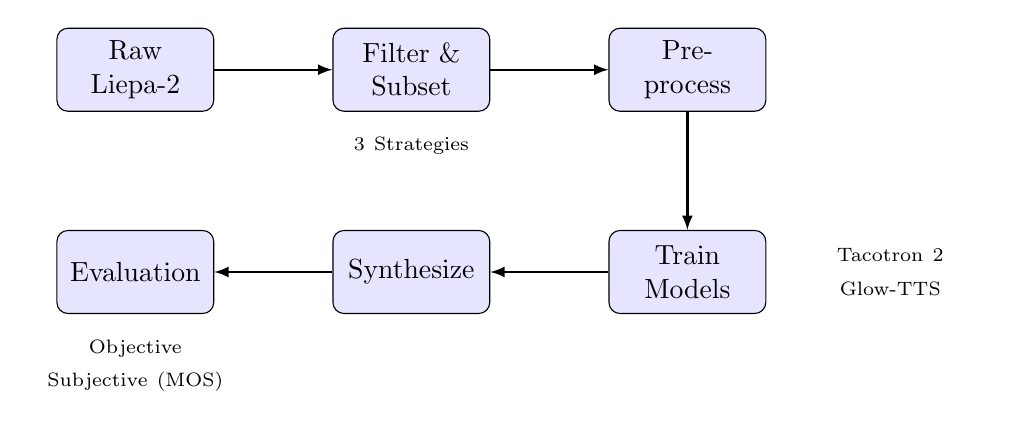
\begin{tikzpicture}[
                  node distance=1.5cm, auto,
                  block/.style={rectangle, draw, fill=blue!10, text width=5em, text centered, rounded corners, minimum height=3em},
                  line/.style={draw, -latex, thick},
                  cloud/.style={draw, ellipse, fill=red!10, node distance=2.5cm, minimum height=2em}
            ]

            % Nodes
            \node [block] (raw) {Raw Liepa-2};
            \node [block, right=of raw] (filter) {Filter \& Subset};
            \node [block, right=of filter] (preproc) {Pre-process};
            \node [block, below=of preproc] (train) {Train Models};
            \node [block, left=of train] (synth) {Synthesize};
            \node [block, left=of synth] (eval) {Evaluation};

            % Edges
            \path [line] (raw) -- (filter);
            \path [line] (filter) -- (preproc);
            \path [line] (preproc) -- (train);
            \path [line] (train) -- (synth);
            \path [line] (synth) -- (eval);

            % Labels
            \node [below=0.2cm of filter, text width=2cm, align=center] {\scriptsize 3 Strategies};
            \node [right=0.2cm of train, text width=2.5cm, align=center] {\scriptsize Tacotron 2\\ Glow-TTS};
            \node [below=0.2cm of eval, text width=2.5cm, align=center] {\scriptsize Objective\\ Subjective (MOS)};
      \end{tikzpicture}
      \caption[Experimental pipeline overview]{Experimental pipeline overview. The process flows from raw corpus selection to comparative evaluation.}\label{fig:pipeline}
\end{figure}

\subsection{Research Design}

To investigate the impact of data distribution on synthesis quality, the
experiments varied the balance between the number of speakers ($N$) and the
amount of data per speaker.

\begin{description}
      \item [Independent Variables:] \hfill
            \begin{itemize}
                  \item \textbf{Data selection strategy:} Three subsets varying in speaker count and duration per speaker (breadth versus depth).
                  \item \textbf{Model architecture:} Tacotron~2 (autoregressive) and Glow-TTS (non-autoregressive).
            \end{itemize}

      \item [Dependent Variables:] \hfill
            \begin{itemize}
                  \item \textbf{Objective metrics:} MCD, $F_0$~RMSE, and attention alignment convergence.
                  \item \textbf{Subjective metrics:} Naturalness ratings via MOS\@.
            \end{itemize}

      \item [Controlled Variables:] \hfill
            \begin{itemize}
                  \item \textbf{Training budget:} Fixed at 22.5 hours of audio data per model.
                  \item \textbf{Training duration:} 90k steps for Tacotron~2 and 180k steps for Glow-TTS, adjusted for convergence characteristics.
                  \item \textbf{Vocoder:} Pre-trained HiFi-GAN (frozen).
                  \item \textbf{Domain:} Read speech (adults only).
            \end{itemize}
\end{description}

\subsection{The Liepa-2 Dataset}

The primary dataset of this study is the \textbf{Liepa-2} Lithuanian speech
corpus~\cite{liepa2project}. The dataset was obtained from the authors upon
request for research purposes. To the best of the author's knowledge, this is
currently the largest freely available annotated multi-speaker Lithuanian
speech dataset. The full corpus contains 1,000 hours of annotated audio from
2,621~unique speakers. Of this, 939~hours are transcribed speech, while the
remaining 61~hours consist of non-speech noise segments. The recordings span
diverse speech styles and contexts, including read speech (audiobooks, studio
recordings, dictaphone) and spontaneous speech (phone, radio, TV), sampled at
16~kHz in 16-bit PCM WAV format.

According to the documentation, the dataset filenames encode metadata about
each recording. These filenames were used to retrieve the following information
about each audio file: lossiness (lossy or raw), speech type (read or
spontaneous), recording type (audiobook, dictaphone, phone, radio, studio, TV),
gender (male or female), age group (0--12, 13--17, 18--25, 26--60, 60+),
speaker ID, recording sequence number, and utterance number.

The documentation notes that speaker IDs are unique only within the context of
an annotator, but not globally across the entire corpus. However, the
documentation claims that duplicate speakers are rare, though not specifically
marked in the dataset. Thus, speaker IDs were treated as globally unique for
the purposes of this study.

\subsubsection{Corpus Analysis and Filtering}

The dataset was analyzed to determine the distribution of audio duration,
sentence length, and speaker distributions across different speech types and
recording conditions.

Analysis revealed that of the 939~hours of transcribed speech, read speech
constitutes the majority (855~hours), while spontaneous speech accounts for
under 9\% (84~hours). Synthesizing spontaneous speech is more challenging due
to disfluencies, high variability, and syntactic conventions different from
those of written language~\cite{szekely2019spontaneous}. Read speech, on the
other hand, is generally more suitable for TTS training due to its consistent
pronunciation and prosody.

Of the read speech, studio recordings account for the largest portion (577
hours, 67\%), followed by dictaphone (220 hours, 25\%) and audiobooks (25
hours, 3\%). The remaining 33 hours (4\%) are from TV, phone, and radio
recordings. The latter three categories of read speech recordings were excluded
due to the potentially less controlled recording conditions, or distinct
acoustic characteristics that could introduce unwanted variability into the
training data. Thus, the focus was placed on the more abundant studio,
dictaphone, and audiobook sources, all of which were deemed more likely to be
recorded in controlled environments favourable for TTS training.

Additionally, it was decided to exclude speakers under 18 years of age to
maintain compatibility with the pre-trained HiFi-GAN vocoder. Speakers in the
0--17 age group constitute a small fraction (76 hours, 8\%) of the total corpus
duration, so their exclusion was not expected to significantly impact the
available training data.

Finally, samples shorter than 1 second or longer than 15 seconds were filtered
out. Samples under 1 second are very short utterances that provide limited
linguistic context. These short samples comprise 32 hours (4\%) of the read
speech data. On the other hand, samples longer than 15 seconds have been found
to cause GPU memory overflows during Tacotron~2 training due to the increased
sequence lengths. Longer samples account for 34 minutes (0.07\%) of the read
speech data.

To summarize, the filtering criteria applied to the Liepa-2 dataset were as
follows:

\begin{itemize}
      \item Speech type: Read speech only
      \item Recording type: Audiobook, Dictaphone, Studio
      \item Age group: Adults only (18--25, 26--60, 60+ age groups)
      \item Duration: Between 1 and 15 seconds
\end{itemize}

After applying these filters, the resulting dataset contained 723 hours of read
speech from 1,794 unique adult speakers. Table~\ref{tab:filtered_liepa2_stats}
summarizes the statistics of the filtered Liepa-2 dataset. A number of speakers
have multiple recording types (e.g., both studio and dictaphone), so the total
unique speaker count is less than the sum across categories.

\begin{table}[htbp]
      \centering
      \caption[Statistics of the filtered Liepa-2 dataset]{Statistics of the filtered Liepa-2 dataset.}\label{tab:filtered_liepa2_stats}
      \small
      \begin{tabular}{llrrrrr}
            \toprule
            \textbf{Source} & \textbf{Sum Duration (h)} & \textbf{Mean Sent.\ Len.\ (char.)} & \textbf{Speakers} & \textbf{Files}   \\
            \midrule
            Audiobook       & 24.32                     & 39.45                              & 50                & 33,826           \\
            Dictaphone      & 188.26                    & 37.12                              & 453               & 256,386          \\
            Studio          & 510.77                    & 42.81                              & 1,303             & 649,651          \\
            \midrule
            \textbf{Total}  & \textbf{723.35}           & \textbf{---}                       & \textbf{1,794}    & \textbf{939,863} \\
            \bottomrule
      \end{tabular}
\end{table}

\subsection{Experimental Training Data Subsets}

The Liepa-2 corpus presents a challenge as most speakers contribute under
30~minutes of audio, while the speaker with the most data has only 2.5~hours of
annotated speech. In order to isolate the impact of data breadth and depth, it
was decided to create controlled training subsets from the filtered Liepa-2
data that vary in the number of speakers and the amount of data per speaker.
However, the duration per speaker within each subset had to be uniform to
prevent speaker imbalance from confounding the results.

The filtered Liepa-2 dataset was analyzed to determine feasible data
configurations. For each gender (male and female), the speakers were sorted by
total available duration. Figure~\ref{fig:speaker_duration} shows the rank
against cumulative duration to visualize the depth versus breadth trade-off. It
was determined that the \textit{15-th} most data-rich male and female speakers
had approximately 47 and 48 minutes of audio, respectively, while the
\textit{180-th} most data-rich speakers had 30 (male) and 34 (female) minutes.
Data depth was clearly the limiting factor, as very few speakers had more than
1~hour of audio.

\begin{figure}[htbp]
      \centering
      \includegraphics[width=\textwidth]{figures/liepa_speaker_duration.png}
      \caption[Speaker duration distribution in the filtered Liepa-2 dataset]{Speaker duration distribution in the filtered Liepa-2 dataset. The plot illustrates the trade-off between the number of speakers (X axis) and available data per speaker (Y axis).}\label{fig:speaker_duration}
\end{figure}

Thus, three training datasets were generated from the filtered Liepa-2 data.
All strategies maintained a fixed total training budget of 22.5 hours. Based on
the speaker duration analysis (Figure~\ref{fig:speaker_duration}), it was
decided that the dataset with the highest depth would have 45~minutes per
speaker, allowing for 30 speakers (15 male, 15 female), and two additional
datasets would contain 60 and 180 speakers, respectively. The configurations
are defined in Table~\ref{tab:data_subsets} and visually represented in
Figure~\ref{fig:data_strategy}.

The validation set was not predefined --- a random 1\% subset of each training
dataset was selected for validation. In order to ensure that different training
jobs on the same dataset used the same validation set, a fixed random seed was
used when sampling the validation data.

\begin{figure}[htbp]
      \centering
      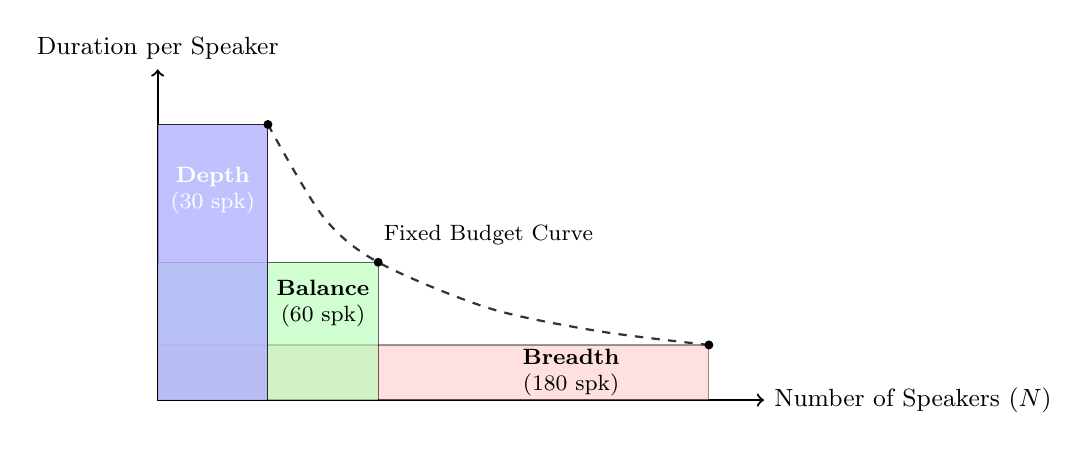
\begin{tikzpicture}[scale=0.7]
            % Axes
            \draw[->, thick] (0,0) -- (11,0) node[right] {\small Number of Speakers ($N$)};
            \draw[->, thick] (0,0) -- (0,6) node[above] {\small Duration per Speaker};

            % Breadth (Wide and Short)
            \draw[fill=red!30, opacity=0.4] (0,0) rectangle (10, 1);
            \node[align=center, font=\footnotesize] at (7.5, 0.5) {\textbf{Breadth}\\(180 spk)};

            % Balance (Medium)
            \draw[fill=green!30, opacity=0.6] (0,0) rectangle (4, 2.5);
            \node[align=center, font=\footnotesize] at (3, 1.75) {\textbf{Balance}\\(60 spk)};

            % Depth (Tall and Narrow)
            \draw[fill=blue!30, opacity=0.8] (0,0) rectangle (2, 5);
            \node[align=center, font=\footnotesize, text=white] at (1, 3.8) {\textbf{Depth}\\(30 spk)};

            % Curve
            \draw[dashed, thick, black!80] plot [smooth] coordinates {(2,5) (3,3.33) (4,2.5) (6,1.67) (8,1.25) (10,1)};

            % Label for the line
            \node[fill=white, inner sep=2pt, font=\footnotesize, sloped] at (6, 3) {Fixed Budget Curve};

            % Dots at the intersection points
            \filldraw (2,5) circle (2pt);
            \filldraw (4,2.5) circle (2pt);
            \filldraw (10,1) circle (2pt);
      \end{tikzpicture}
      \caption[Visual representation of the data strategies]{Visual representation of the data strategies. The area of each rectangle (Total Audio) remains constant ($\approx$ 22.5 hours), illustrating the trade-off between speaker diversity (Breadth) and data density (Depth).}\label{fig:data_strategy}
\end{figure}

Only speakers with at least the required minimum duration for the specific
subset were eligible for selection (e.g., at least 45 minutes for the
30-speaker set). For each selected speaker, a fixed set of utterances (10 per
speaker) was held out for testing. The durations listed in
Table~\ref{tab:data_subsets} represent idealized targets, with actual durations
varying slightly due to the discrete nature of utterance selection.

\begin{table}[htbp]
      \centering
      \caption[Experimental training data subsets]{Experimental training data subsets. Total duration is constant, while speaker count ($N$) and duration per speaker vary inversely.}\label{tab:data_subsets}
      \begin{tabular}{ccc}
            \toprule
            \textbf{Number of Speakers ($N$)} & \textbf{Time/Speaker} & \textbf{Total Time} \\
            \midrule
            30                                & 45.0 min              & 22.5 hours          \\
            60                                & 22.5 min              & 22.5 hours          \\
            180                               & 7.5 min               & 22.5 hours          \\
            \bottomrule
      \end{tabular}
\end{table}

To ensure fair evaluation, speaker sets were nested: the 30 speakers in the
30-speaker set were included in the 60-speaker set, which were in turn included
in the 180-speaker set. An exact 50/50 male-female split was maintained in all
datasets to avoid gender bias.

This nesting strategy ensured that the `core' 30 speakers were present in every
model. This enabled a direct, side-by-side comparison of synthesis quality for
the exact same target voices, effectively isolating the impact of the trainset
composition without confounding factors from speaker identity.

The datasets were generated using a custom Python script. In order to ensure
that each speaker would have at least the required minimum duration, speakers
were first filtered based on their total available audio. From each eligible
speaker, a random subset of utterances was selected until the cumulative
duration met or exceeded the target.

The statistics of the actual training datasets are summarized in
Table~\ref{tab:final_data_stats}. The slight variations in total utterance
count and total word count could be attributed to speakers having varying
speaking rates and utterance lengths --- these differences are minimal and not
expected to significantly impact the results. The minimum and maximum durations
within each dataset are very similar, confirming that there is no significant
speaker-level imbalance.

\begin{table}[htbp]
      \centering
      \caption[Final statistics of the experimental training datasets]{Final statistics of the experimental training datasets.}\label{tab:final_data_stats}
      \begin{tabular}{lrrrr}
            \toprule
            \textbf{Speakers} & \textbf{Utterances} & \textbf{Total Words} & \textbf{Unique Words} & \textbf{Duration per Speaker (s), Min / Max} \\
            \midrule
            30                & 29,091              & 164,347              & 46,138                & 2700.2 / 2705.3                              \\
            60                & 30,372              & 163,883              & 46,746                & 1350.1 / 1356.5                              \\
            180               & 30,493              & 168,738              & 49,581                & 450.0 / 458.0                                \\
            \bottomrule
      \end{tabular}
\end{table}

\subsection{Data Preparation}

\subsubsection{Text Normalization and Accentuation}

In the absence of a high-quality, context-aware G2P converter for Lithuanian,
this study focused on grapheme-based TTS synthesis. The raw transcripts from
the Liepa-2 dataset were pre-processed to standardize the text. A prior
study~\cite{kasparaitis2023investigation} has shown that text normalization has
a significant impact on grapheme-based TTS quality for Lithuanian.

Raw Liepa-2 transcripts are largely normalized --- numbers, dates,
abbreviations, and acronyms are expanded. An analysis of the raw text revealed
that some annotators did not use any punctuation (e.g., commas, periods), while
others used punctuation consistently. Otherwise, the transcripts were of high
quality. Due to the high volume of training samples, no manual correction of
transcripts was performed. Some examples of raw transcripts are presented
below:

\begin{quote}
      \textit{``Berželio Sodų šeštoji septyniolika''} (ordinal and number written out) \\
      \textit{``Anoniminis darbdavys pasiūlė šimtas penkiasdešim tūkstančių eurų už tai''} (number 150,000 written out) \\
      \textit{``ir kabindavo makaronus apie vė dė vė didybę ir galingumą''} (acronym VDV written as it was pronounced) \\
      \textit{``nenumanau šypsodamasis atsakė jis bet spėju kad netrukus sužinosime''} (punctuation omitted) \\
\end{quote}

However, additional normalization was required to standardize the text for
grapheme-based TTS training. The following normalization steps were applied:

\begin{enumerate}
      \item \textbf{Cleaning:} Rare and non-standard punctuation was mapped to a standard set (.,-?!) and remaining extraneous characters were removed.
      \item \textbf{Whitespace:} Consecutive whitespace characters were collapsed, and leading/trailing whitespace was trimmed.
      \item \textbf{Accentuation:} Raw text was processed using \textbf{Kirčiuoklis}~\cite{kirciuoklis} for automatic stress assignment. The stress marks were decomposed into separate characters (`´' for acute, ``' for grave, `~' for circumflex) and inserted immediately after the accented grapheme.
      \item \textbf{Lowercasing:} All text was converted to lowercase to reduce the vocabulary size.
      \item \textbf{Letter substitution:} Non-Lithuanian letters were replaced with equivalents (`q' $\to$ `k', `w' $\to$ `v', `x' $\to$ `ks').
\end{enumerate}

The accentuation step required dealing with ambiguity. As discussed in the
literature review, the Lithuanian language has many homographs that can have
different stress patterns, depending on the word's meaning and context.
Kirčiuoklis, being a word dictionary-based tool, does not take into account the
context of the word, and returns all possible accentuation options for
homographs. Of 406 thousand unique words in the entire filtered Liepa-2 corpus,
72\% (293 thousand) had a single accentuation option, 18\% (75 thousand) had
none (e.g., proper nouns (`Trento'), foreign words (`siut'), typos and
neologisms (`babkių')), and 9\% (38 thousand) had multiple accentuation options
(e.g., `namo', `pažintų'). In order to avoid introducing incorrect accents into
the training data, only unambiguous words were accented --- the rest of the
words were left unaccentuated, instead relying on the models to infer prosody
from context. Listening tests revealed that implementing Kirčiuoklis-based
accentuation moderately improved the prosody of synthesized speech, especially
for certain complex words. Overall, 82\% of words in the training datasets were
accentuated.

A few examples of raw and normalized text pairs are presented in
Table~\ref{tab:text_normalization}.

\begin{table}[htbp]
      \centering
      \caption[Examples of text normalization and accentuation]{Examples of text normalization and accentuation.}\label{tab:text_normalization}
      \begin{tabular}{p{8cm} p{8cm}}
            \toprule
            \textbf{Raw Text}                                           & \textbf{Normalized Text}                                   \\
            \midrule
            \texttt{Antrasis vyras – gerokai jaunesnis}                 & \texttt{antra`sis vy´ras - gero´kai jaune`snis}            \\
            \texttt{(...) pusšimtį kilogramų Extasy}                    & \texttt{(...) pu`sšimtį kilogra\char`\~mų ekstasy}         \\
            \texttt{Visa tai atskleidžiama „Karaliaus Lyro“ pradžioje,} & \texttt{visa tai atskleidžiama karaliaus lyro pradžioje`,} \\
            \bottomrule
      \end{tabular}
\end{table}

As a result of these normalization steps, the character vocabulary size was
reduced from 140~characters to 41~characters. The final alphabet used for
training contains only lowercase Lithuanian letters, stress marks, space, and
basic punctuation:
\begin{center}
      \texttt{a ą b c č d e ę ė f g h i į y j k l m n o p r s š t u ų ū v z ž ´ ` \textasciitilde{} (space) . , - ? !}
\end{center}

\subsubsection{Audio Preprocessing}

Audio recordings were resampled from their original \textbf{16,000 Hz} to
\textbf{22,050 Hz}. While resampling to a higher frequency does not add new
information, the resampling was performed to match the pre-trained HiFi-GAN
vocoder described in the \textbf{Vocoder} section below. Leading and trailing
silence was trimmed. Acoustic features were extracted using the parameters in
Table~\ref{tab:audio_params}.

\begin{table}[htbp]
      \centering
      \caption[Mel-spectrogram extraction parameters]{Mel-spectrogram extraction parameters.}\label{tab:audio_params}
      \begin{tabular}{lr}
            \toprule
            \textbf{Parameter}       & \textbf{Value}        \\
            \midrule
            Sampling rate            & 22,050 Hz             \\
            FFT size                 & 1024 samples (46 ms)  \\
            Hop length               & 256 samples (11.6 ms) \\
            Window length            & 1024                  \\
            Mel-spectrogram channels & 80                    \\
            Frequency range          & 0--8000 Hz            \\
            Pre-emphasis             & 0.98                  \\
            \bottomrule
      \end{tabular}
\end{table}

A complete list of audio parameters is presented in the
Appendix~\ref{appendix:audio_params}.

\subsection{Model Architectures}

For each data selection strategy, two acoustic models were trained: an
autoregressive Tacotron~2 and a non-autoregressive Glow-TTS\@. These
architectures were chosen due to their popularity and to represent two modern
TTS paradigms, namely seq2seq attention-based generation and flow-based
parallel generation. VITS, despite its state-of-the-art quality, was not
included due to substantially higher computational requirements required for
training, and VITS being a combination of Glow-TTS acoustic model and HiFi-GAN
vocoder, which is already covered in this study. It was decided to isolate the
acoustic model performance, before considering end-to-end models like VITS in
future work. All models were implemented using the \textbf{Coqui
      TTS}~\cite{coqui2021} framework.

\subsubsection{Vocoder}

\textbf{HiFi-GAN}~\cite{kong2020hifi} was chosen as the vocoder for this study due to its widespread adoption and ability to generate high-fidelity audio with significantly lower computational latency compared to autoregressive vocoders (e.g., WaveNet~\cite{oord2016wavenet}, WaveGlow).

More specifically, a HiFi-GAN model pre-trained on the multi-speaker VCTK
corpus~\cite{veaux2019cstr} was used. The vocoder's weights were frozen to
isolate the performance differences to the acoustic models only. As described
in the \textbf{Audio Preprocessing} section, the acoustic parameters of both
Tacotron~2 and Glow-TTS were matched to those of the pre-trained HiFi-GAN to
ensure compatibility.

\subsubsection{Tacotron~2}

The autoregressive model used was \textbf{Tacotron~2}, modified with DCA to
improve alignment stability for long-form utterances, on which the standard
location-sensitive attention was observed to struggle.

The architecture details are displayed in Table~\ref{tab:tacotron_arch}.

\begin{table}[htbp]
      \centering
      \caption[Tacotron~2 with DCA architecture details]{Tacotron~2 with DCA architecture details.}\label{tab:tacotron_arch}
      \begin{tabular}{lr}
            \toprule
            \textbf{Component}  & \textbf{Configuration}                    \\
            \midrule
            Text Encoder        & 3-layer convolution + Bi-LSTM (512 units) \\
            Attention Mechanism & Dynamic Convolution Attention (DCA)       \\
            Separate Stopnet    & True                                      \\
            Decoder             & 2-layer LSTM (1024 units)                 \\
            Speaker Embedding   & 512 dimensions                            \\
            \bottomrule
      \end{tabular}
\end{table}

The training objective $\mathcal{L}_{T2}$ is a weighted sum of auxiliary
losses:
\begin{equation}
      \mathcal{L}_{T2} = \mathcal{L}_{L1} + \mathcal{L}_{Post} + \lambda_{SSIM}(\mathcal{L}_{SSIM}) + \lambda_{attn}(\mathcal{L}_{Guided}) + \lambda_{stop}(\mathcal{L}_{Stop})
\end{equation}
Where $\mathcal{L}_{Guided}$ enforces diagonal attention alignment, critical for preventing repeating or skipping words in long-form synthesis.

\subsubsection{Glow-TTS}

The non-autoregressive model used was \textbf{Glow-TTS}, a flow-based
architecture. The main architectural hyperparameters used in this study are
detailed in Table~\ref{tab:glow_arch}.

\begin{table}[htbp]
      \centering
      \caption[Glow-TTS architecture details]{Glow-TTS architecture details.}\label{tab:glow_arch}
      \begin{tabular}{lr}
            \toprule
            \textbf{Component}        & \textbf{Configuration} \\
            \midrule
            Encoder Type              & Rel. Pos. Transformer  \\
            Encoder Layers            & 6                      \\
            Encoder Heads             & 2                      \\
            Encoder Hidden Dimensions & 192                    \\
            Decoder Hidden Dimensions & 192                    \\
            Decoder Flow Blocks       & 12                     \\
            Decoder Block Layers      & 4                      \\
            Decoder Kernel Size       & 5                      \\
            Duration Predictor        & 256 hidden channels    \\
            Speaker Embedding         & 512 dimensions         \\
            \bottomrule
      \end{tabular}
\end{table}

The objective function maximizes the log-likelihood of the data:
\begin{equation}
      \log P_X(x|c) = \sum_{j=1}^{T_{mel}} \log \left| \det \frac{\partial z_j}{\partial x_j} \right| + \sum_{j=1}^{T_{mel}} \log \mathcal{N}(z_j; \mu, \sigma)
\end{equation}
Additionally, a duration predictor is trained via MSE loss $\mathcal{L}_{Dur}$ to predict phoneme durations.

\subsubsection{Speaker Conditioning}

In this work, learnable speaker embeddings (Look-Up Tables) are used for both
Tacotron~2 and Glow-TTS models. The primary reason is that this study focuses
on synthesis for a known set of speakers, where learnable embeddings can
outperform pre-computed vectors~\cite{arik2017deep}. They allow each model to
learn a latent representation for each voice that reflects the features most
relevant for each model architecture, rather than features used specifically to
distinguish between speakers in a classification task. This eliminates the
information bottleneck or noise introduced by an external verification model.

In Tacotron~2, the speaker embedding is broadcast-concatenated with the output
of the text encoder. This conditions the decoder at every time step, allowing
the autoregressive mechanism to factor in speaker identity when generating each
Mel-spectrogram frame.

In Glow-TTS, the embedding conditions the flow-based decoder. Specifically, it
is applied as global conditioning within the affine coupling layers of the flow
steps~\cite{kim2020glowtts}. This allows the model to learn a multi-speaker
distribution by adapting the flow transformation function to map the
speaker-agnostic latent representation to the target speaker's Mel-spectrogram.

\subsection{Model Training Configurations}

\subsubsection*{Environment and Framework}

Experiments were conducted on a personal workstation equipped with an AMD Epyc
7642 CPU, 256 GB RAM, and NVIDIA GeForce RTX 3090 (24 GB) GPU\@. The software
environment included Ubuntu 25.04, Python 3.13.3, Coqui TTS v0.27.2, and CUDA
13.0 for GPU acceleration. The pipeline was automated via Make, with separate
steps for data preprocessing, model training, inference, and synthesized sample
deployment to an evaluation web app.

The exact Python environment configuration is provided in the accompanying
GitHub repository, file \texttt{pyproject.toml}.

In the TTS training stage, the validation loss was evaluated every epoch
($\approx$ 450 steps) using a held-out (randomly selected) 1\% validation
split. The best model checkpoint was selected based on the lowest validation
loss.

\subsubsection*{Tacotron~2 Configuration}

The model optimization utilized a composite loss function consisting of Decoder
L1 loss ($\alpha=0.25$), Post-net L1 loss ($\alpha=0.25$), Decoder and Post-net
SSIM losses ($\alpha=0.25$ each), Guided Attention loss ($\alpha=5.0$), and a
weighted Stop token loss (weight $= 15.0$).

The default learning rate scheduler in Coqui TTS, NoamLR, was experimentally
found to cause high gradient values, instability, and slow convergence for
Tacotron~2. The original Tacotron~2 implementation~\cite{shen2018natural} used
an exponential decay schedule with a starting learning rate of 0.001, which at
50,000 steps began exponentially decaying to $10^{-5}$. Coqui TTS
configurations do not support starting gradual exponential decay at a specific
step. Additionally, the original Tacotron~2 learning rate of 0.001 was found to
cause numerical instability and exploding gradients in preliminary experiments,
hence the lower starting learning rate of 0.0005 was chosen. To approximate a
decay profile similar to the original Tacotron~2 paper, a MultiStepLR scheduler
with stepwise decay of 0.5 every 10,000 steps (20k, 30k, \dots, 70k) was used
instead, starting from an initial learning rate of $0.0005$, and reaching
$\approx 7.81 \times 10^{-8}$ at 70,000 steps. Unlike the original Tacotron~2
paper, no warmup period was used, as it was found to be unnecessary for
training from scratch.

This schedule yielded more stable training and faster convergence, as observed
in TensorBoard plots. Additionally, the RAdam optimizer~\cite{liu2021variance}
was used instead of the default Adam, as it provided more stable convergence in
preliminary experiments. The total training duration was set to 200 epochs
($\approx$ 90,000 steps), which took approximately 22 hours per model to train.
The main training hyperparameters are shown in Table~\ref{tab:tacotron_config}.

\begin{table}[h!]
      \centering
      \caption[Tacotron~2 with DCA training configuration]{Tacotron~2 with DCA training configuration.}\label{tab:tacotron_config}
      \begin{tabular}{lr}
            \toprule
            \textbf{Parameter}    & \textbf{Value}                                        \\
            \midrule
            Validation split      & 1\%                                                   \\
            Batch size            & 64                                                    \\
            Initial Learning Rate & 0.0005                                                \\
            Optimizer             & RAdam                                                 \\
            LR schedule           & MultiStepLR (Decay 0.5 at steps 20k, 30k, \dots, 70k) \\
            Max epochs            & 200 ($\approx$ 90,000 steps)                          \\
            Reduction factor      & 2                                                     \\
            Number of speakers    & 30 / 60 / 180                                         \\
            \bottomrule
      \end{tabular}
\end{table}

\subsubsection*{Glow-TTS Configuration}

The Glow-TTS model was trained using Negative Log-Likelihood (NLL) for the flow
decoder and a monotonic alignment search. Glow-TTS converged stably with the
NoamLR scheduler used in the original implementation, but required a higher
number of epochs (400 epochs, or $\approx$ 180,000 steps) for convergence. The
loss function was a combination of NLL loss for the flow-based decoder, and MSE
for the duration predictor.

Based on preliminary experiments, the models were trained for 300 epochs
($\approx$ 135,000 steps) with the NoamLR scheduler, followed by an additional
100 epochs ($\approx$ 45,000 steps) with an exponentially decaying learning
rate (ExponentialLR scheduler), with a starting LR of 0.001, decay rate 0.95
every epoch, final LR $\approx$ 0.00008. This two-stage schedule yielded small
but consistent improvements in all tracked loss metrics on the training and
validation sets, as observed in TensorBoard plots. The total training time per
model was approximately 25 hours. The configuration is shown in
Table~\ref{tab:glow_config}.

\begin{table}[h!]
      \centering
      \caption[Glow-TTS training configuration]{Glow-TTS training configuration.}\label{tab:glow_config}
      \begin{tabular}{lr}
            \toprule
            \textbf{Parameter}         & \textbf{Value}                                  \\
            \midrule
            Validation split           & 1\%                                             \\
            Batch size                 & 64                                              \\
            Maximum Learning Rate      & 0.001                                           \\
            Optimizer                  & RAdam                                           \\
            LR scheduler               & NoamLR (300 epochs), ExponentialLR (100 epochs) \\
            Warmup steps (NoamLR)      & 4000                                            \\
            Decay rate (ExponentialLR) & 0.95 per epoch                                  \\
            Max epochs                 & 300 + 100 ($\approx$ 180,000 steps)             \\
            Number of speakers         & 30 / 60 / 180                                   \\
            \bottomrule
      \end{tabular}
\end{table}

\subsection{Evaluation Protocol}

The synthesized speech from the trained models was evaluated using a
combination of objective and subjective metrics.

\subsubsection{Model Convergence}

Alignment stability during training was monitored via attention alignment
plots, provided by the TensorBoard~\cite{abadi2016tensorflow} integration in
Coqui TTS\@.

The \textbf{attention alignment plots} were generated during every epoch, and
inspected regularly. A failure to converge to a diagonal alignment would
indicate that the model has failed to learn the text-to-audio mapping. This was
especially relevant for the 180-speaker scenario to detect convergence failures
caused by data sparsity.

\subsubsection{Objective Evaluation}

A held-out test set of 60 standardized sentences (using 6 seen speakers) was
used to calculate objective metrics. The metrics selected for evaluation were
MCD and $F_0$~RMSE, as they capture different aspects of synthesis quality:
spectral fidelity and intonation accuracy, respectively.
PESQ~\cite{rix2001perceptual} was considered for inclusion, but ultimately not
used due to its sensitivity to slight temporal misalignments between
synthesized and reference audio --- a known limitation when evaluating
generative TTS models that produce valid but non-aligned prosody.

\textbf{Mel-Cepstral Distortion (MCD):} MCD~\cite{kubichek1993mel} evaluates the timbre and spectral envelope of synthesized speech. It measures the difference between the Mel-frequency cepstral coefficients of the synthesized and reference speech. A lower MCD value indicates closer spectral similarity, i.e., better timbre reconstruction. The MCD is defined as:
\begin{equation}
      \text{MCD} = \frac{10}{\ln 10} \sqrt{2 \sum_{n=1}^{K} (c_n^{\text{synth}} - c_n^{\text{ref}})^2}
\end{equation}
where $c_n^{\text{synth}}$ and $c_n^{\text{ref}}$ are the $n$-th coefficients of the synthesized and reference frames, respectively, and $K$ is the number of coefficients (here: 24).

\textbf{Fundamental Frequency Root Mean Square Error ($F_0$~RMSE):} $F_0$~RMSE measures the Root Mean Square Error between the fundamental frequency ($F_0$) contours of the synthesized and reference speech. Lower $F_0$~RMSE values indicate better pitch accuracy, i.e., closer intonation reproduction. $F_0$~RMSE is defined as:
\begin{equation}
      \text{RMSE}_{F_0} = \sqrt{\frac{1}{T} \sum_{t=1}^{T} (F_0^{\text{synth}}(t) - F_0^{\text{ref}}(t))^2}
\end{equation}
$F_0^{\text{synth}}(t)$ and $F_0^{\text{ref}}(t)$ are the fundamental frequency values at time $t$ for
synthesized and ground truth speech, respectively, and $T$ is the total number of frames where both signals are voiced. Lower values indicate more accurate intonation.

\subsubsection{Subjective Evaluation}

Subjective evaluation was conducted via a web-based listening test employing a
\textbf{Latin square design} to mitigate order and repetition biases. An
application was developed specifically for this study, using the \textbf{Flask}
web framework, \textbf{Google Cloud Run} app hosting service, \textbf{Google
      Cloud Storage} for audio file hosting, and \textbf{PostgreSQL} for storing
ratings. The complete source code is available in the accompanying GitHub
repository linked in the Appendix~\ref{appendix:github}, folder
\texttt{tts\_rating\_app}.

Naturalness was rated using the standard 5-point MOS scale. The test samples
were generated using the 6 experimental models plus a human ground truth
baseline. The test samples were 60 sentences from the held-out test set: for 6
randomly selected speakers (3 male, 3 female, from the 30-speaker subset), 10
held-out sentences were selected from the Liepa-2 dataset, resulting in a total
of 60 test samples.

The participants were native Lithuanian speakers recruited through university
networks and social media platforms. Each rater evaluated a randomized block of
sentences, ensuring balanced exposure to all models and sentences.

\subsubsection{Rating Procedure}

Raters accessed the web application via a public
URL\@\footnote{\url{https://tts-rating-app-6128007182.europe-west1.run.app/}}.
The application required raters to sign in using their Google account
(Appendix~\ref{appendix:app_screens}, Figure~\ref{fig:app_screens}~(a)). This
was done to automatically assign a unique internal identifier and prevent
duplicate submissions. Upon signing in, raters were presented with a welcome
page detailing the study's purpose, data usage, confidentiality assurances, and
explaining the rating procedure (Appendix~\ref{appendix:app_screens},
Figure~\ref{fig:app_screens}~(b)). Only those who provided informed consent
could proceed to the evaluation.

Once the evaluation began, raters were presented with audio samples one at a
time, along with the corresponding text prompt
(Appendix~\ref{appendix:app_screens}, Figure~\ref{fig:app_screens}~(c)). Raters
listened to each sample and rated its naturalness on a scale from 1 (Bad) to 5
(Excellent). Audio samples could be replayed multiple times as needed before
submitting each rating. Submitted ratings were immediately stored in a
PostgreSQL database, and the next sample was presented. A progress bar
indicated the number of samples rated out of the expected total (60 samples per
rater). Once a rater completed all assigned samples, they were thanked for
their participation and informed that their responses had been recorded
(Appendix~\ref{appendix:app_screens}, Figure~\ref{fig:app_screens}~(d)).

\subsubsection{Statistical Analysis}

Collected MOS ratings were screened for outliers and inconsistencies. Only
raters who completed 100\% of their assigned samples were included in the final
analysis. The mean MOS ratings and 95\% confidence intervals (CI) were computed
for each model and data subset.

The 95\% confidence intervals were calculated using the Student's
t-distribution:
\begin{equation}
      CI = \bar{x} \pm t_{0.975, N-1} \cdot \frac{s}{\sqrt{N}}
\end{equation}
where $\bar{x}$ is the arithmetic mean of the ratings, $s$ is the sample
standard deviation, $N$ is the number of ratings, and $t_{0.975, N-1}$ is the
critical t-value for a two-tailed 95\% confidence level with $N-1$ degrees of
freedom.

To determine whether the observed differences in MOS were statistically
significant, a one-way Analysis of Variance (ANOVA) was conducted. The
F-statistic is calculated as the ratio of between-group variance to
within-group variance:
\begin{equation}
      F = \frac{MS_{between}}{MS_{within}}
\end{equation}

Upon finding significant main effects (i.e., $p < 0.05$), Tukey's Honestly
Significant Difference (HSD) post-hoc test was applied to identify specific
pairwise differences. Two means are considered significantly different if their
absolute difference exceeds the HSD critical value:
\begin{equation}
      HSD = q_{\alpha, k, \nu} \sqrt{\frac{MS_{within}}{N}}
\end{equation}
where $q$ is the critical value from the Studentized range distribution for
significance level $\alpha$, $k$ groups, and $\nu$ degrees of freedom, and $N$
is the number of samples per group. All statistical tests were performed at a
significance level of $\alpha=0.05$.

\subsection{Qualitative Analysis}

A qualitative analysis of these speakers' original recordings, transcripts, and
synthesis outputs was conducted by the study author. The primary goal was to
identify possible factors related to synthesis quality. This included examining
aspects such as audio quality, voice characteristics, and prosody. Particular
attention was paid to speakers exhibiting extreme synthesis quality (both high
and low) to identify potential contributing factors.

%%%%%%%%%%%%%%%%%%%%%%%%%%%%%%%%%%%%%%%%%%%%%%%%%%%%%%%%%%%%%%%%%%%%%%%%%%%%%%%%
%% Results and analysis
%%%%%%%%%%%%%%%%%%%%%%%%%%%%%%%%%%%%%%%%%%%%%%%%%%%%%%%%%%%%%%%%%%%%%%%%%%%%%%%%
\section{Results and Analysis}

This chapter presents the quantitative and qualitative findings of the study.
The performance of the autoregressive (Tacotron~2) and non-autoregressive
(Glow-TTS) models was analyzed across the three data subsets defined in
Chapter~3: 30 speakers (45 minutes per speaker), 60 speakers (22.5 minutes per
speaker), and 180 speakers (7.5 minutes per speaker).

\subsection{Objective Evaluation}

Table~\ref{tab:objective_results} summarizes the MCD and $F_0$~RMSE on the
held-out test set.

\begin{table}[htbp]
      \centering
      \caption[Objective synthesized speech evaluation results]{Objective synthesized speech evaluation results. Lower is better. Bold indicates best performance per architecture.}\label{tab:objective_results}
      \begin{tabular}{llcc}
            \toprule
            \textbf{Model} & \textbf{Speaker Count ($N$)} & \textbf{MCD (dB)} & \textbf{$F_0$~RMSE (Hz)} \\
            \midrule
            \multirow{3}{*}{Tacotron~2}
                           & 30                           & 9.58              & 31.28                    \\
                           & 60                           & \textbf{9.55}     & \textbf{30.49}           \\
                           & 180                          & 9.63              & 31.06                    \\
            \midrule
            \multirow{3}{*}{Glow-TTS}
                           & 30                           & \textbf{9.90}     & 37.86                    \\
                           & 60                           & 10.00             & 36.18                    \\
                           & 180                          & 9.98              & \textbf{35.69}           \\
            \bottomrule
      \end{tabular}
\end{table}

Both model architectures showed significant robustness to the data composition
strategy in terms of objective metrics. Minimal intra-model variations were
observed for MCD --- the highest difference between data subsets was under 0.1
dB, with Tacotron~2 achieving its best MCD on the 60-speaker subset, and
Glow-TTS on the 30-speaker subset. Similarly, $F_0$~RMSE varied only slightly
across datasets for both architectures --- less than 1.0 Hz difference was
observed for Tacotron~2, and under 2.2 Hz for Glow-TTS\@. The 180-speaker
configuration achieved the best $F_0$~RMSE for Glow-TTS (35.69 Hz), suggesting
that increased speaker diversity did not harm pitch modeling, and may have even
helped generalization. Across all data subsets, Tacotron~2 moderately but
consistently outperformed Glow-TTS in MCD (between 0.32--0.45 dB lower) and
$F_0$~RMSE (between 4.63--6.58 Hz lower).

\subsubsection{Alignment Convergence}

\textbf{Tacotron~2} demonstrated no visible sensitivity to data sparsity. On all subsets, the attention mechanism converged to a clear diagonal alignment within 10k steps. While there were occasional minor misalignments during training, by the end of training, all models exhibited stable alignments on all test sentences.

As seen in Figure~\ref{fig:alignments}, the attention maps for Tacotron~2
remain stable across all data subsets, indicating robust alignment learning
even in low-resource conditions. Glow-TTS, utilizing MAS, also converged
successfully across all three subsets.

\begin{figure}[htbp]
      \centering

      % Tacotron 2 row
      \begin{subfigure}{0.32\textwidth}
            \centering
            \includegraphics[width=\textwidth]{figures/taco2_alignment_30spk.png}
            \caption{Tacotron~2, 30 speakers}
      \end{subfigure}
      \hfill
      \begin{subfigure}{0.32\textwidth}
            \centering
            \includegraphics[width=\textwidth]{figures/taco2_alignment_60spk.png}
            \caption{Tacotron~2, 60 speakers}
      \end{subfigure}
      \hfill
      \begin{subfigure}{0.32\textwidth}
            \centering
            \includegraphics[width=\textwidth]{figures/taco2_alignment_180spk.png}
            \caption{Tacotron~2, 180 speakers}
      \end{subfigure}

      \vspace{0.5em}

      % Glow-TTS row
      \begin{subfigure}{0.32\textwidth}
            \centering
            \includegraphics[width=\textwidth]{figures/glow_alignment_30spk.png}
            \caption{Glow-TTS, 30 speakers}
      \end{subfigure}
      \hfill
      \begin{subfigure}{0.32\textwidth}
            \centering
            \includegraphics[width=\textwidth]{figures/glow_alignment_60spk.png}
            \caption{Glow-TTS, 60 speakers}
      \end{subfigure}
      \hfill
      \begin{subfigure}{0.32\textwidth}
            \centering
            \includegraphics[width=\textwidth]{figures/glow_alignment_180spk.png}
            \caption{Glow-TTS, 180 speakers}
      \end{subfigure}

      \caption[Attention alignments across architectures and data subsets]{Attention alignments after training: Tacotron~2 (a--c) and Glow-TTS (d--f) across 30, 60, and 180 speaker configurations. All models exhibit clear monotonic alignments, indicating successful convergence.}\label{fig:alignments}
\end{figure}

\subsubsection{Pitch and Spectral Accuracy}

Tacotron~2 consistently outperformed Glow-TTS in pitch accuracy ($F_0$~RMSE),
achieving values around 31~Hz compared to Glow-TTS's 36~Hz. Furthermore,
Tacotron~2 achieved slightly lower MCD scores on all subsets, suggesting it
captures fine-grained spectral details better than the flow-based decoder. The
raters noted that Glow-TTS outputs often sounded monotone, though the predicted
pitch contours had sudden jumps and drops in the fundamental frequency,
possibly due to Glow-TTS not having an explicit pitch predictor.

Spectral analysis confirms the objective metrics. As illustrated in an example
of Mel-spectrogram comparison Figure~\ref{fig:spectrogram_comparison},
Tacotron~2 captures visibly more fine-grained spectral details and intonation
contours more accurately than Glow-TTS, which tends to produce flatter, less
dynamic outputs.

\begin{figure}[htbp]
      \centering
      \begin{subfigure}{0.32\textwidth}
            \centering
            \includegraphics[width=\textwidth]{figures/mel_sp_gt.png}
            \caption{Ground truth}
      \end{subfigure}
      \hfill
      \begin{subfigure}{0.32\textwidth}
            \centering
            \includegraphics[width=\textwidth]{figures/mel_sp_taco2.png}
            \caption{Tacotron~2 output}
      \end{subfigure}
      \hfill
      \begin{subfigure}{0.32\textwidth}
            \centering
            \includegraphics[width=\textwidth]{figures/mel_sp_glow.png}
            \caption{Glow-TTS output}
      \end{subfigure}
      \caption[Mel-spectrogram comparison of Tacotron~2 and Glow-TTS outputs]{Comparison of ground truth Mel-spectrogram (a),
            Tacotron~2 (b) and Glow-TTS (c) outputs for the same speaker and input text. Note how Glow-TTS produces flatter pitch contours.}\label{fig:spectrogram_comparison}
\end{figure}

\subsection{Subjective Evaluation}

Naturalness was evaluated via a Latin square design listening test with 24
native speakers, who rated samples from all six experimental models plus the
ground truth on a 5-point MOS scale. 3 raters were excluded for incomplete
submissions, resulting in a final count of 21 raters. Each rater evaluated 60
samples, yielding a total of 1,260 ratings (21 raters $\times$ 60 samples). The
results are presented in Table~\ref{tab:mos_results}.

\begin{table}[htbp]
      \centering
      \caption[MOS results per model and data subset]{MOS results per model and data subset with 95\% confidence intervals. Bold indicates best performance per architecture.}\label{tab:mos_results}
      \begin{tabular}{llc}
            \toprule
            \textbf{Model}        & \textbf{Speaker count ($N$)} & \textbf{MOS (95\% CI)} \\
            \midrule
            \textbf{Ground Truth} & ---                          & $\bm{4.84 \pm 0.06}$   \\
            \midrule
            \multirow{3}{*}{Tacotron~2}
                                  & 30                           & $3.11 \pm 0.16$        \\
                                  & 60                           & $\bm{3.12 \pm 0.17}$   \\
                                  & 180                          & $3.03 \pm 0.18$        \\
            \midrule
            \multirow{3}{*}{Glow-TTS}
                                  & 30                           & $2.13 \pm 0.12$        \\
                                  & 60                           & $2.18 \pm 0.15$        \\
                                  & 180                          & $2.03 \pm 0.14$        \\
            \bottomrule
      \end{tabular}
\end{table}

\subsubsection*{Statistical Significance}

The one-way ANOVA revealed significant differences among the six experimental
models ($F(5, 1074) = 46.8490, p < 0.001$). Tukey's HSD post-hoc analysis
identified 9 significant pairwise differences at $\alpha=0.05$. The full list
of tested pairs and their significance is provided in
Appendix~\ref{appendix:anova}, Table~\ref{tab:anova_results}. When analyzing
the significant differences, all of them were between different model
architectures (Tacotron~2 vs. Glow-TTS) rather than data subsets within the
same architecture.

Notably, within each architecture, there were no statistically significant
differences between the three data composition strategies (30, 60, or 180
speakers). While the 60-speaker configuration achieved marginally higher mean
MOS scores for both models (3.12 for Tacotron~2, 2.18 for Glow-TTS), and the
180-speaker setup showed slights decreases (3.03 for Tacotron~2, 2.03 for
Glow-TTS), these differences were not statistically significant. ANOVA tests
conducted separately for Tacotron~2 ($p = 0.71$) and Glow-TTS ($p = 0.34$) also
failed to reject the null hypothesis that speaker count affects MOS, indicating
that data composition did not have a measurable impact on naturalness within
the tested range.

\subsubsection*{Architecture Comparison}

The MOS results revealed a significant performance gap between the two
architectures.

\textbf{Tacotron~2} achieved a consistently higher synthesis quality in the study, with the 60-speaker configuration scoring $3.12 \pm 0.17$. Listeners noted that Tacotron~2 produces highly expressive prosody for some of the speakers. Increasing the speaker count to 180 caused a moderate, albeit statistically insignificant, drop in naturalness to $3.03 \pm 0.18$.

\textbf{Glow-TTS} lagged behind Tacotron~2 in naturalness, with the 60-speaker configuration scoring $2.18 \pm 0.15$. The listeners reported that Glow-TTS seemed to have strong robotic artifacts, and was at times unintelligible. This was especially pronounced in the 180-speaker condition where the MOS dropped to $2.03 \pm 0.14$.

\subsubsection*{Speaker MOS Analysis}

An analysis of individual speakers' MOS scores was conducted to identify any
patterns related to speaker identity. Table~\ref{tab:speaker_mos} summarizes
the average MOS per speaker and model architecture.

\begin{table}[ht]
      \centering
      \caption[MOS results per speaker and model architecture]{MOS results per speaker and model architecture with 95\% confidence intervals. Bold indicates highest score per architecture.}\label{tab:speaker_mos}
      \begin{tabular}{lcc}
            \toprule
            \textbf{Speaker ID} & \textbf{Tacotron~2 MOS} & \textbf{Glow-TTS MOS} \\
            \midrule
            AS009               & $\bm{4.17 \pm 0.20}$    & $\bm{2.61 \pm 0.23}$  \\
            IS031               & $3.26 \pm 0.20$         & $2.13 \pm 0.19$       \\
            IS038               & $3.48 \pm 0.21$         & $2.51 \pm 0.19$       \\
            MS052               & $2.26 \pm 0.17$         & $1.88 \pm 0.16$       \\
            VP131               & $2.43 \pm 0.19$         & $1.93 \pm 0.16$       \\
            VP427               & $2.92 \pm 0.22$         & $1.60 \pm 0.14$       \\
            \bottomrule
      \end{tabular}
\end{table}

Notably, speaker \textbf{AS009} consistently received the highest ratings
across both models (Tacotron~2 MOS\@: 4.17, Glow-TTS MOS\@: 2.61), suggesting
that certain speaker or dataset characteristics (e.g., clear articulation,
consistent recording quality, or clean transcripts) may facilitate better
synthesis quality. On the other hand, speakers like \textbf{MS052} and
\textbf{VP427} scored significantly lower, indicating potential data quality
issues or inherent speaker traits (e.g., strong accents, background noise) that
challenge the TTS models.

\subsection{Qualitative Analysis}

Consistent with the MOS findings, the author observed no subjective correlation
between synthesis naturalness and the data composition strategy (speaker
count). Thus, any observations below apply across all data subsets.

\begin{itemize}
      \item \textbf{AS009 (low male voice):} Source audio is clear, neutral accent; transcripts are unpunctuated. \\
            \textit{Tacotron~2:} Highly natural output with accurate prosody. Closely resembled the target speaker. \\
            \textit{Glow-TTS:} Suffered from pitch instability, frequently shifting into a falsetto-like register (approximately one octave higher than the target).

      \item \textbf{IS031 (low female voice):} Source audio is clear, neutral accent; transcripts are unpunctuated. \\
            \textit{Tacotron~2:} Good prosody, though minor robotic artifacts were audible. \\
            \textit{Glow-TTS:} Intelligible but had intonation issues --- it was either monotone, or had pitch issues (jumping up by several semitones, or dipping into bass range).

      \item \textbf{IS038 (average male voice):} Source audio is clear, neutral accent; transcripts are unpunctuated. \\
            \textit{Tacotron~2:} Prosody was accurate, but minor voice artifacts (`scratchy' quality, higher-frequency noise) were present. \\
            \textit{Glow-TTS:} Intelligible, but failed to capture the speaker's timbre. Exhibited pitch issues similar to IS031.

      \item \textbf{MS052 (average female voice):} Source audio sounds muffled, likely due to room acoustics, neutral accent; transcripts are punctuated. \\
            \textit{Tacotron~2:} Mostly good prosody and intonation, but a muffled voice quality, more pronounced than in the original audio. \\
            \textit{Glow-TTS:} Mostly intelligible, but the voice did not match the original audio. Monotone, often very low-pitched intonation in the male range.

      \item \textbf{VP131 (young, higher female voice):} Source audio has slight reverberation, neutral accent; transcripts are punctuated. \\
            \textit{Tacotron~2:} Intelligible, good prosody, but the voice sounded muffled and older than the target speaker. \\
            \textit{Glow-TTS:} Mostly intelligible and matched the true voice quite well, but had monotone intonation and `scratchy' voice quality. Interestingly, no pitch jump artifacts were observed for this speaker.

      \item \textbf{VP427 (young, higher male voice):} Source audio is clear, but slight accent on certain phonemes; transcripts are punctuated. \\
            \textit{Tacotron~2:} Good prosody, but had moderate artifacts in the high-frequency range. \\
            \textit{Glow-TTS:} Significantly distorted, with a `scratchy' voice quality, monotone intonation, and artifacts in the high-frequency range.
\end{itemize}

A recurring issue with Glow-TTS was the generation of unnatural pitch jumps and
octave errors. To investigate this, the Glow-TTS outputs were re-synthesized
using the Griffin-Lim vocoder instead of HiFi-GAN\@.

While the Griffin-Lim samples remained monotone, the prevalence of sudden pitch
jumps decreased. However, the synthesized voices had strong harmonics,
indicating poor spectral quality. This suggests that Glow-TTS may have
generated ambiguous fundamental frequency contours with excessive harmonic
content. When fed into HiFi-GAN, these ambiguities may have confused the
vocoder, causing it to `flip' between different harmonics, interpreting them as
the fundamental frequency.

These observations underline the significant role of audio quality and speaker
characteristics in determining synthesis quality. Speakers with clean
recordings free from reverberation (e.g., AS009, IS031) yielded higher
synthesis quality across both architectures. On the other hand, speakers with
slightly muffled audio (MS052, VP131) or idiosyncratic vocal features (VP427)
resulted in degraded performance. Glow-TTS outputs exhibited pronounced issues
with intonation, often producing monotone speech, or significant pitch jumps to
unnatural ranges, which were not observed in Tacotron~2 outputs.

\subsection{Discussion}

The results provide several insights into the effects of data composition and
model architecture on multi-speaker TTS quality in low-resource settings.

Firstly, objective metrics ($F_0$~RMSE, MCD) exhibited minor variations across
the data strategies, with no clear trend indicating a substantial performance
degradation for higher speaker counts. The maximum observed differences within
each architecture were under 0.1 dB for MCD and under 2.2 Hz for $F_0$~RMSE\@.
Glow-TTS achieved its best $F_0$~RMSE in the 180-speaker configuration,
suggesting that increased speaker diversity did not harm pitch modeling, and
may have even helped generalization.

Secondly, the autoregressive Tacotron~2 moderately but consistently
outperformed the non-autoregressive Glow-TTS in both objective ($F_0$~RMSE,
MCD) and subjective (MOS) metrics, across all dataset configurations.
Tacotron~2 achieved a peak MOS score of \textbf{3.12} in the 60-speaker setup,
while Glow-TTS reached a maximum MOS of \textbf{2.18}. The consistent
superiority of Tacotron~2 suggests that in low-resource constraints, the
stability of its explicit alignment mechanism may outweigh the benefits of
Glow-TTS and MAS\@.

Data composition had no statistically significant effect on synthesis quality
within either architecture. One-way ANOVA tests for each model separately
failed to detect significant differences between the 30-, 60-, and 180-speaker
configurations (Tacotron~2: $p = 0.71$; Glow-TTS\@: $p = 0.34$). Although small
numerical variations existed (60-speaker slightly higher, 180-speaker slightly
lower), these were not beyond statistical noise. This null result suggests that
within the tested range, the total data volume (22.5 hours) acts as the primary
constraint, and that the specific distribution strategy (breadth versus depth)
does not meaningfully impact naturalness. Instead, per-speaker data quality
appears to be the dominant factor.

Indeed, speaker-specific analysis revealed that certain speakers consistently
yielded significantly higher synthesis quality across models and data
strategies. Within both architectures, speaker \textbf{AS009} consistently
received the highest ratings (Tacotron~2 MOS\@: 4.17, Glow-TTS MOS\@: 2.61),
while speakers like \textbf{MS052} and \textbf{VP131} scored significantly
lower, the highest MOS being only 2.43 for Tacotron~2 and 1.93 for Glow-TTS\@.
Qualitative analysis suggests that speaker characteristics and data quality
play a crucial role in TTS performance.

%%%%%%%%%%%%%%%%%%%%%%%%%%%%%%%%%%%%%%%%%%%%%%%%%%%%%%%%%%%%%%%%%%%%%%%%%%%%%%%%
%% Conclusion
%%%%%%%%%%%%%%%%%%%%%%%%%%%%%%%%%%%%%%%%%%%%%%%%%%%%%%%%%%%%%%%%%%%%%%%%%%%%%%%%
\section{Conclusion}

This thesis set out to measure the effects of training data composition on the
quality of multi-speaker TTS models for the Lithuanian language under a fixed
resource budget. All research objectives were achieved. Three training datasets
were constructed and pre-processed from the Liepa-2 corpus, each containing a
total of 22.5 hours of speech, but varying in the number of speakers and amount
of data per speaker: 30 speakers with 45 minutes each, 60 speakers with 22.5
minutes each, and 180 speakers with 7.5 minutes each. An autoregressive
(Tacotron~2) and a non-autoregressive (Glow-TTS) architecture was trained on
each dataset. The synthesis quality of the trained models was evaluated using
objective metrics ($F_0$~RMSE, MCD) and a subjective MOS listening test using a
web-based evaluation application developed for this study.

\subsubsection*{Summary of Findings}

The experimental results do not support the initial hypothesis that data depth
is more important than breadth for multi-speaker synthesis quality. Instead,
the findings indicate that data composition had \textbf{no statistically
      significant effect} on synthesis quality within either architecture.
Statistical analysis confirmed that when the total data volume is held constant
at 22.5 hours, the choice between 30, 60, or 180 speakers does not meaningfully
affect subjective naturalness. Objective metrics (MCD, $F_0$~RMSE) similarly
showed minimal variation across data subsets for both architectures.

Despite the low data volume per speaker in the 180-speaker subset (7.5
minutes), both architectures successfully converged. This indicates that 7.5
minutes of data per speaker is above the `critical threshold' required to learn
stable alignments and synthesize intelligible speech for Lithuanian,
contradicting concerns that low-depth settings would prevent convergence.

Regarding the architecture, Tacotron~2 consistently outperformed Glow-TTS
across all data configurations. Subjective feedback indicated that Tacotron~2
produced more natural and expressive speech, while Glow-TTS outputs suffered
from robotic intonation and artifacts, described as `scratchy voice'. It is
unclear what specific architectural, language, or dataset features led to this
gap, but it could be attributed to Glow-TTS lacking an explicit pitch
predictor.

Finally, speaker-specific analysis revealed that certain speakers consistently
yielded higher-quality synthesis regardless of the data strategy. Qualitative
analysis suggested that these differences may stem from audio quality issues
(e.g., muffled recordings, room acoustics) or speaker traits (e.g., accents,
vocal characteristics).

\subsubsection*{Contributions}

This work makes several contributions to the field of multi-speaker TTS\@.

Firstly, it provides an empirical evaluation of the trade-off between speaker
breadth and depth for training multi-speaker TTS models for Lithuanian. The
primary finding --- a null result --- reveals that modern architectures are
insensitive to data composition within the tested range (30--180 speakers) when
total volume is held constant. This negative result is scientifically valuable:
it suggests that practitioners working with low-resource languages should
prioritize maximizing total data volume and ensuring high per-speaker quality
rather than optimizing the breadth-depth balance.

Additionally, this study establishes benchmark results for Tacotron~2 and
Glow-TTS on the Lithuanian Liepa-2 corpus in several multi-speaker settings. It
demonstrates that Tacotron~2 can achieve reasonable synthesis quality with as
little as 7.5 minutes of data per speaker when using learnable speaker
embeddings.

Finally, the development of a web-based MOS evaluation application for
Lithuanian TTS provides a reusable tool for future subjective evaluations in
this language. The application source code is made publicly available for reuse
and adaptation.~\footnote{See Appendix~\ref{appendix:github} for the GitHub
      repository link.}

\subsubsection*{Limitations}

The first limitation of this work is the language and dataset specificity. The
experiments were exclusively focused on the Lithuanian language and read speech
from the Liepa-2 speech corpus. Therefore, the findings may not generalize to
other languages, datasets, or speech styles.

Secondly, the fixed training budget of 22.5 hours is a practical constraint and
may not reflect performance in higher-resource settings (e.g., 100 hours or
more).

Finally, as discussed in the qualitative analysis, the training data had
variable quality across speakers. The synthesis quality of certain speakers
(MS052, VP131, VP427) was consistently rated as poor regardless of data
strategy or model architecture.

\subsubsection*{Future Work}

There are several potential directions for future research building on this
study. First, replicating the experiments on different languages and datasets
would help validate the cross-lingual generalizability of the findings. It
would be valuable to test languages with phonetic or prosodic characteristics
distinct from Lithuanian (e.g., non-phonemic orthographies like English or
highly regular orthographies like Italian) to determine if the observed
insensitivity to data composition holds. Additionally, exploring a wider range
of data budgets could provide insights into scaling effects; for instance, a
100-hour budget could reveal different or more pronounced trade-offs than the
22.5-hour setting used here.

Furthermore, future work should focus on data quality and selection strategies.
If a cleaner multi-speaker dataset for Lithuanian becomes available,
replicating the experiments on such a dataset could help isolate the effects of
data composition from recording artifacts. This would likely achieve higher
synthesis quality overall. In the absence of new data, automated quality
assessment could be used to filter out recordings with low signal-to-noise
ratios or excessive reverberation. Additionally, given the significant
variability in synthesis quality observed between speakers --- even among those
with subjectively good audio quality --- future research could aim to
systematically identify and prioritize speakers with favourable characteristics
(e.g., vocal clarity, intonation patterns). Such targeted selection of
high-quality voices may yield greater improvements than simply increasing
dataset size or performing manual curation.

Finally, extending the study to include more TTS architectures, such as VITS or
FastSpeech~2, would provide a broader understanding of how different model
types respond to data composition strategies. This could help identify
architectures that possess greater robustness to low-depth data settings
compared to the Tacotron~2 and Glow-TTS models evaluated here.

%%%%%%%%%%%%%%%%%%%%%%%%%%%%%%%%%%%%%%%%%%%%%%%%%%%%%%%%%%%%%%%%%%%%%%%%%%%%%%%%
%% References
%%%%%%%%%%%%%%%%%%%%%%%%%%%%%%%%%%%%%%%%%%%%%%%%%%%%%%%%%%%%%%%%%%%%%%%%%%%%%%%%
\section{References}

\printbibliography[heading=none]

\sectionnonum{Appendix 1: AI Tool Usage}\label{appendix:ai_usage}

This appendix documents the use of Generative AI tools in the preparation of
this thesis. Table~\ref{tab:ai_tools} lists the specific versions and access
dates of the tools employed.

\begin{table}[ht]
      \centering
      \caption[List of AI tools used]{List of AI tools used}\label{tab:ai_tools}
      \begin{tabular}{lll}
            \toprule
            \textbf{Tool Name}                                      & \textbf{Models/Versions}       & \textbf{Usage Dates}   \\ \midrule
            Google Gemini~\cite{google2026gemini}                   & 2.5 Flash, 3.0 Flash           & 2025-09-02--2026-01-03 \\
            \midrule
            GitHub Copilot Code Generation~\cite{github2026copilot} & Claude Haiku 4--4.5            & 2025-09-02--2026-01-03 \\
                                                                    & Claude Sonnet 4--4.5           &                        \\
            \midrule
            GitHub Copilot Code Completion~\cite{github2026copilot} & Plugin versions 1.5.53--1.5.62 & 2025-09-02--2026-01-03 \\
            \bottomrule
      \end{tabular}
\end{table}

\subsection*{Text Drafting and Refinement}

\noindent\textbf{Tool used:} Google Gemini~\cite{google2026gemini} 2.5 Flash, 3.0 Flash \\
\noindent\textbf{Extent of usage:} The tool was used for drafting specific subsections of the literature review and methodology, suggesting citations, refining the author's original text (paraphrasing, grammar correction), and providing critical feedback on logical flow.

\noindent\textbf{Method of usage:}
Interaction was text-based via the chat interface. An author's prompt would be
submitted, and the AI-generated response was reviewed and edited by the author.

\begin{itemize}
      \item \textit{Drafting literature review, methodology:} Generating the initial outline and draft text for specific subsections of the literature review based on provided key points, unstructured notes, and reference lists. \\
            \textit{Prompt pattern:} ``Based on my notes below and this list of references, draft a latex outline / literature review subsubsection on [Topic]: --- Notes: [Insert Notes] --- References: [Insert References]''
      \item \textit{Citation suggestions:} The author provided a topic or claim, and the AI suggested relevant academic references to support it. All suggested references were manually verified for existence and actual relevance. \\
            \textit{Prompt pattern:} ``Find academic references for these claims: --- [Insert Claims]''
      \item \textit{Refinement and paraphrasing:} The author pasted original drafts to improve clarity. \\
            \textit{Prompt pattern:} ``Review the following MSc thesis draft for academic tone, grammar errors, and sentence structure. Paraphrase only where unclear. Do not change the technical meaning unless necessary: [Insert Text]''
      \item \textit{Critique:} Used to identify gaps in argumentation. \\
            \textit{Prompt pattern:} ``Act as a thesis reviewer. Read the following thesis subsection, identify notable logical gaps, unclear explanations, missing citations. Provide critique and suggest improvement. --- [Insert Text]''
\end{itemize}

\noindent\textbf{Author contribution:}
The author conducted the primary literature review, selected all references, and defined the structure of the review. All AI-suggested drafts were fact-checked against original sources. The author accepted or rejected the AI critiques and phrasing or structure. Over 90\% of AI suggestions were rejected, with the remaining 10\% being used as templates for updates or basis for rephrasing.

\subsection*{Code Completion and Generation}

\noindent\textbf{Tool used:} GitHub Copilot~\cite{github2026copilot} \\
\noindent\textbf{Extent of usage:} Used for code completion, generating boilerplate code for the MOS rating application, drafting Python code for figure generation, data preprocessing, and dataset generation scripts.

\noindent\textbf{Method of usage:}
Usage occurred within the Visual Studio Code environment via the GitHub Copilot
plugin. The author wrote code comments or partial code snippets, and Copilot
Code Completion provided real-time suggestions for completing lines or generating functions.
Additionally, the Copilot Code Generation feature was used to generate drafts of larger Python code blocks based on descriptive prompts.

\begin{itemize}
      \item \textit{Inline code completion:} In the Visual Studio Code editor, GitHub Copilot provided real-time predictive text for line completions based on the active file context (variable names, function definitions). This was used primarily for coding efficiency in Python scripts for data preprocessing, analysis, and MOS rating application development.
      \item \textit{Generative chat:} The author described functionality to generate/alter specific code blocks for dataset generation and MOS app features. \\
            \textit{Prompt pattern:} ``Add static consent form that displays study information below, saves user agreement in session storage, and prevents proceeding to /rate if not agreed. Use flask and jinja2 --- study information: [Insert Study Info]''
      \item \textit{Figure drafting:} The author provided data structures and requested plotting code. \\
            \textit{Prompt pattern:} ``For pd.DataFrame df with columns [`model', `rating', `user\_email'] plot grouped bar chart using matplotlib, place the legend outside plot area on the upper right''
\end{itemize}

\noindent\textbf{Author contribution:}
The author designed the overall model training pipeline, software architecture of the MOS rating app and defined all functional requirements. AI was used strictly as an implementation assistant to speed up generation of boilerplate code and routine functions. The author manually reviewed, tested, and debugged all generated code. The author verified that the generated figures accurately represented the underlying data and manually adjusted visual styles as needed.

\sectionnonum{Appendix 2: Source Code}\label{appendix:github}

All steps outlined in this work were implemented in Python, SQL, or JavaScript
using open-source libraries. The complete source code for data preprocessing,
model training, inference, and evaluation is available in the author's GitHub
repository\@\footnote{\url{https://github.com/spacegrapefruit/msc-thesis}}.

The structure of the repository is as follows:
\begin{itemize}
      \item \texttt{configs/}: Configuration files for model hyperparameters and training settings.
      \item \texttt{data/}: Not included due to size constraints; contains raw and preprocessed audio data.
      \item \texttt{latex/}: LaTeX source files for the thesis document.
      \item \texttt{Makefile}: Build instructions for running experiments and generating results.
      \item \texttt{notebooks/}: Jupyter notebooks for exploratory data analysis and visualization.
      \item \texttt{pyproject.toml}: Python project configuration file, specifying package dependencies.
      \item \texttt{python/}: Python scripts for data preprocessing, model training, and evaluation.
      \item \texttt{training\_output/}: Training logs, checkpoints (not included due to size constraints), and TensorBoard summaries.
      \item \texttt{tts\_rating\_app/}: Source code for the web-based MOS rating application.
\end{itemize}

The repository relies on the raw Liepa-2 corpus~\cite{liepa2project}, which is
not included due to size constraints. Liepa-2 is not publicly available due to
the sheer size of the dataset ($> 100GB$). It was obtained from the authors
upon request for research purposes.

\sectionnonum{Appendix 3: MOS Rating Application Interface}\label{appendix:app_screens}

This appendix presents the complete user interface of the web-based MOS
evaluation application used for the perceptual study. The application guides
raters through four main screens: login, consent, rating, and completion.

\begin{figure}[htbp]
      \centering
      \begin{subfigure}{0.47\textwidth}
            \centering
            \includegraphics[width=\textwidth]{figures/app_login.png}
            \caption{Login screen}
      \end{subfigure}
      \hfill
      \begin{subfigure}{0.47\textwidth}
            \centering
            \includegraphics[width=\textwidth]{figures/app_consent.png}
            \caption{Consent screen}
      \end{subfigure}

      \vspace{1em}

      \begin{subfigure}{0.47\textwidth}
            \centering
            \includegraphics[width=\textwidth]{figures/app_rating.png}
            \caption{Rating screen}
      \end{subfigure}
      \hfill
      \begin{subfigure}{0.47\textwidth}
            \centering
            \includegraphics[width=\textwidth]{figures/app_thankyou.png}
            \caption{Completion screen}
      \end{subfigure}

      \caption[Web application interface screens]{Web application interface: (a) login requiring Google authentication, (b) consent screen with study information and MOS instructions, (c) rating screen with text prompt and audio player, (d) completion screen thanking participants.}\label{fig:app_screens}
\end{figure}

\sectionnonum{Appendix 4: Audio Preprocessing Parameters}\label{appendix:audio_params}

The following Mel-spectrogram extraction parameters were used by all models
(Tacotron~2, Glow-TTS, and HiFi-GAN vocoder):

\begin{table}[ht]
      \centering
      \caption[Complete Mel-spectrogram extraction parameters]{Complete Mel-spectrogram extraction parameters.}\label{tab:audio_params_full}
      \begin{tabular}{lr}
            \toprule
            \textbf{Parameter}      & \textbf{Value} \\
            \midrule
            fft\_size               & 1024           \\
            win\_length             & 1024           \\
            hop\_length             & 256            \\
            frame\_length\_ms       & null           \\
            frame\_shift\_ms        & null           \\
            stft\_pad\_mode         & ``reflect''    \\
            sample\_rate            & 22050          \\
            resample                & false          \\
            preemphasis             & 0.98           \\
            ref\_level\_db          & 20             \\
            do\_sound\_norm         & false          \\
            log\_func               & ``np.log10''   \\
            do\_trim\_silence       & true           \\
            trim\_db                & 60             \\
            do\_rms\_norm           & false          \\
            db\_level               & null           \\
            power                   & 1.5            \\
            griffin\_lim\_iters     & 60             \\
            num\_mels               & 80             \\
            mel\_fmin               & 0.0            \\
            mel\_fmax               & 8000.0         \\
            spec\_gain              & 20             \\
            do\_amp\_to\_db\_linear & true           \\
            do\_amp\_to\_db\_mel    & true           \\
            pitch\_fmax             & 640.0          \\
            pitch\_fmin             & 1.0            \\
            signal\_norm            & true           \\
            min\_level\_db          & -100           \\
            symmetric\_norm         & true           \\
            max\_norm               & 4.0            \\
            clip\_norm              & true           \\
            stats\_path             & null           \\
            \bottomrule
      \end{tabular}
\end{table}

\sectionnonum{Appendix 5: ANOVA Statistical Test Details}\label{appendix:anova}

This appendix provides the full list of tested model pairs and the significance
of their mean MOS differences.

\begin{table}[htbp]
      \centering
      \caption[Tukey's HSD post-hoc test results]{Tukey's HSD post-hoc test results for pairwise comparisons of MOS scores between all model and data composition combinations.}\label{tab:anova_results}
      \begin{tabular}{llrrrrr}
            \toprule
            Model A          & Model B          & Mean Diff. & p-adj    & Lower     & Upper    & Reject \\
            \midrule
            Glow-030spk      & Glow-060spk      & 0.050000   & 0.997700 & -0.266600 & 0.366600 & False  \\
            Glow-030spk      & Glow-180spk      & -0.100000  & 0.946100 & -0.416600 & 0.216600 & False  \\
            Glow-030spk      & Tacotron2-030spk & 0.977800   & 0.000000 & 0.661200  & 1.294300 & True   \\
            Glow-030spk      & Tacotron2-060spk & 0.994400   & 0.000000 & 0.677900  & 1.311000 & True   \\
            Glow-030spk      & Tacotron2-180spk & 0.900000   & 0.000000 & 0.583400  & 1.216600 & True   \\
            Glow-060spk      & Glow-180spk      & -0.150000  & 0.755200 & -0.466600 & 0.166600 & False  \\
            Glow-060spk      & Tacotron2-030spk & 0.927800   & 0.000000 & 0.611200  & 1.244300 & True   \\
            Glow-060spk      & Tacotron2-060spk & 0.944400   & 0.000000 & 0.627900  & 1.261000 & True   \\
            Glow-060spk      & Tacotron2-180spk & 0.850000   & 0.000000 & 0.533400  & 1.166600 & True   \\
            Glow-180spk      & Tacotron2-030spk & 1.077800   & 0.000000 & 0.761200  & 1.394300 & True   \\
            Glow-180spk      & Tacotron2-060spk & 1.094400   & 0.000000 & 0.777900  & 1.411000 & True   \\
            Glow-180spk      & Tacotron2-180spk & 1.000000   & 0.000000 & 0.683400  & 1.316600 & True   \\
            Tacotron2-030spk & Tacotron2-060spk & 0.016700   & 1.000000 & -0.299900 & 0.333200 & False  \\
            Tacotron2-030spk & Tacotron2-180spk & -0.077800  & 0.981800 & -0.394300 & 0.238800 & False  \\
            Tacotron2-060spk & Tacotron2-180spk & -0.094400  & 0.957500 & -0.411000 & 0.222100 & False  \\
            \bottomrule
      \end{tabular}
\end{table}

\end{document}
